\documentclass[compress]{beamer}
\usepackage{ifthen,verbatim}

\newcommand{\isnote}{}
\xdefinecolor{lightyellow}{rgb}{1.,1.,0.25}
\xdefinecolor{darkblue}{rgb}{0.1,0.1,0.7}

%% Uncomment this to get annotations
%% \def\notes{\addtocounter{page}{-1}
%%            \renewcommand{\isnote}{*}
%% 	   \beamertemplateshadingbackground{lightyellow}{white}
%%            \begin{frame}
%%            \frametitle{Notes for the previous page (page \insertpagenumber)}
%%            \itemize}
%% \def\endnotes{\enditemize
%% 	      \end{frame}
%%               \beamertemplateshadingbackground{white}{white}
%%               \renewcommand{\isnote}{}}

%% Uncomment this to not get annotations
\def\notes{\comment}
\def\endnotes{\endcomment}

\setbeamertemplate{navigation symbols}{}
\setbeamertemplate{headline}{\mbox{ } \hfill
\begin{minipage}{5.5 cm}
\vspace{-0.75 cm} \small
\end{minipage} \hfill
\begin{minipage}{4.5 cm}
\vspace{-0.75 cm} \small
\begin{flushright}
\ifthenelse{\equal{\insertpagenumber}{1}}{}{Jim Pivarski \hspace{0.2 cm} \insertpagenumber\isnote/\pageref{numpages}}
\end{flushright}
\end{minipage}\mbox{\hspace{0.2 cm}}\includegraphics[height=1 cm]{../cmslogo} \hspace{0.1 cm} \includegraphics[height=1 cm]{../tamulogo} \hspace{0.01 cm} \vspace{-1.05 cm}}

\begin{document}
\begin{frame}
\vfill
\begin{center}
\textcolor{darkblue}{\Large Muon Alignment without RPC-hit Bias}

\vfill
\begin{columns}
\column{0.3\linewidth}
\begin{center}
\large
Aysen Tatarinov

Vadim Khotilovich

\textcolor{darkblue}{\it Jim Pivarski}

Alexei Safonov
\end{center}
\end{columns}

\begin{columns}
\column{0.3\linewidth}
\begin{center}
\scriptsize
{\it Texas A\&M University}
\end{center}
\end{columns}

\vfill
31 May, 2010

\end{center}
\end{frame}

%% \begin{notes}
%% \item This is the annotated version of my talk.
%% \item If you want the version that I am presenting, download the one
%% labeled ``slides'' on Indico (or just ignore these yellow pages).
%% \item The annotated version is provided for extra detail and a written
%% record of comments that I intend to make orally.
%% \item Yellow notes refer to the content on the {\it previous} page.
%% \item All other slides are identical for the two versions.
%% \end{notes}

\small

\begin{frame}
\frametitle{Pablo's Grand Unified Theory}
\framesubtitle{of Muon Track Residuals Mysteries}
\textcolor{red}{Cause of nearly all of our problems: RPC hits were being included in alignment track refits, biasing the residuals (should be tracker hits only)}

\scriptsize
\begin{itemize}\setlength{\itemsep}{0.1 cm}
\item \textcolor{gray}{Sawtooth effect: why are there discontinuities at DT borders?}

\textcolor{gray}{\it Because RPC borders are at the same place as DT borders}

\item \textcolor{gray}{Why does it depend on momentum, like an input-track bias?}

\textcolor{gray}{\it Because the input tracks are biased--- by the RPCs, not tracker}

\item \textcolor{gray}{Why do we see it most strongly in ME1/2 with collisions muons (new)?}

\textcolor{gray}{\it Because that's where the RPCs are in the endcap}

\item \textcolor{gray}{Why does tracker weak-mode effect have a characteristic scale of
  100~GeV/$c$, even with a scale-invariant tracker weak mode?}

\textcolor{gray}{\it Because the distance of the RPCs to the beamline, their
  resolution, and the CMS magnetic field set a characteristic scale of
  about 100~GeV/$c$, not the tracker weak mode}

\item \textcolor{gray}{Why does Reference-Target disagree with Sasha Spiridonov's global
  cross-alignment (also track-based)?}

\textcolor{gray}{\it The cross-alignment algorithm performed a fit
  at the level of standAloneMuons, not residuals, so it was much less
  affected by RPC hits ($\sigma_{RPC} \gg \sigma_{DT}$).}
\end{itemize}
\end{frame}

\begin{frame}
\frametitle{Avoid overlap with Pablo's talk}

\begin{columns}
\column{0.49\linewidth}
\hfill 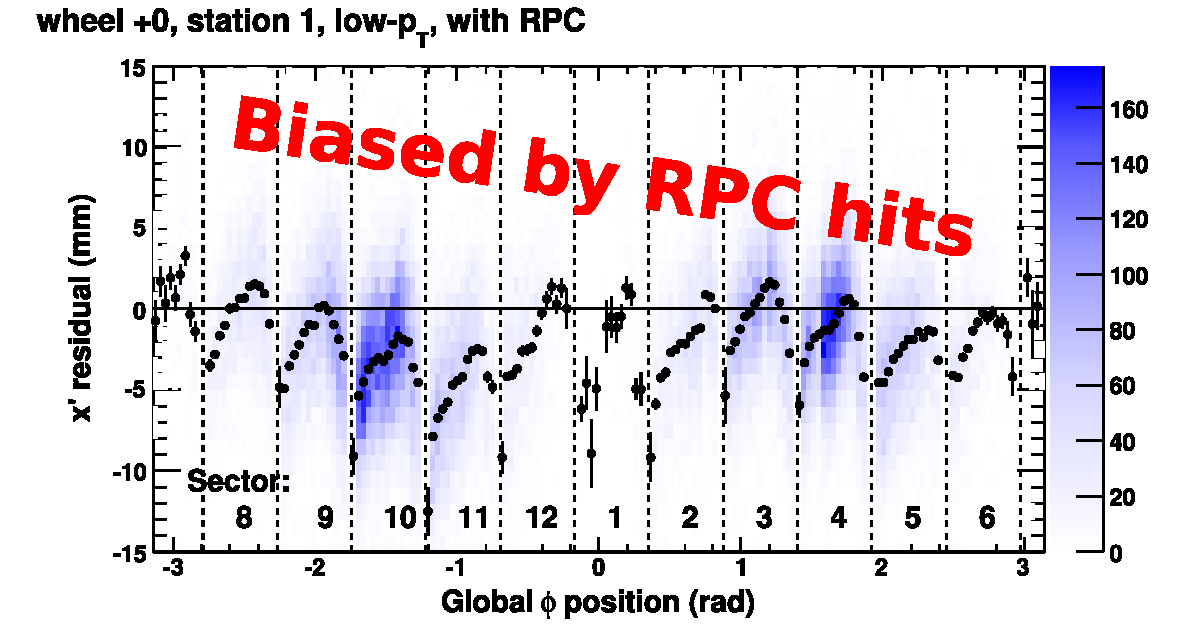
\includegraphics[width=0.9\linewidth]{sawtoothexample_x_low_withrpc.pdf}

\column{0.02\linewidth}
$\mathbf{\to}$

\column{0.49\linewidth}
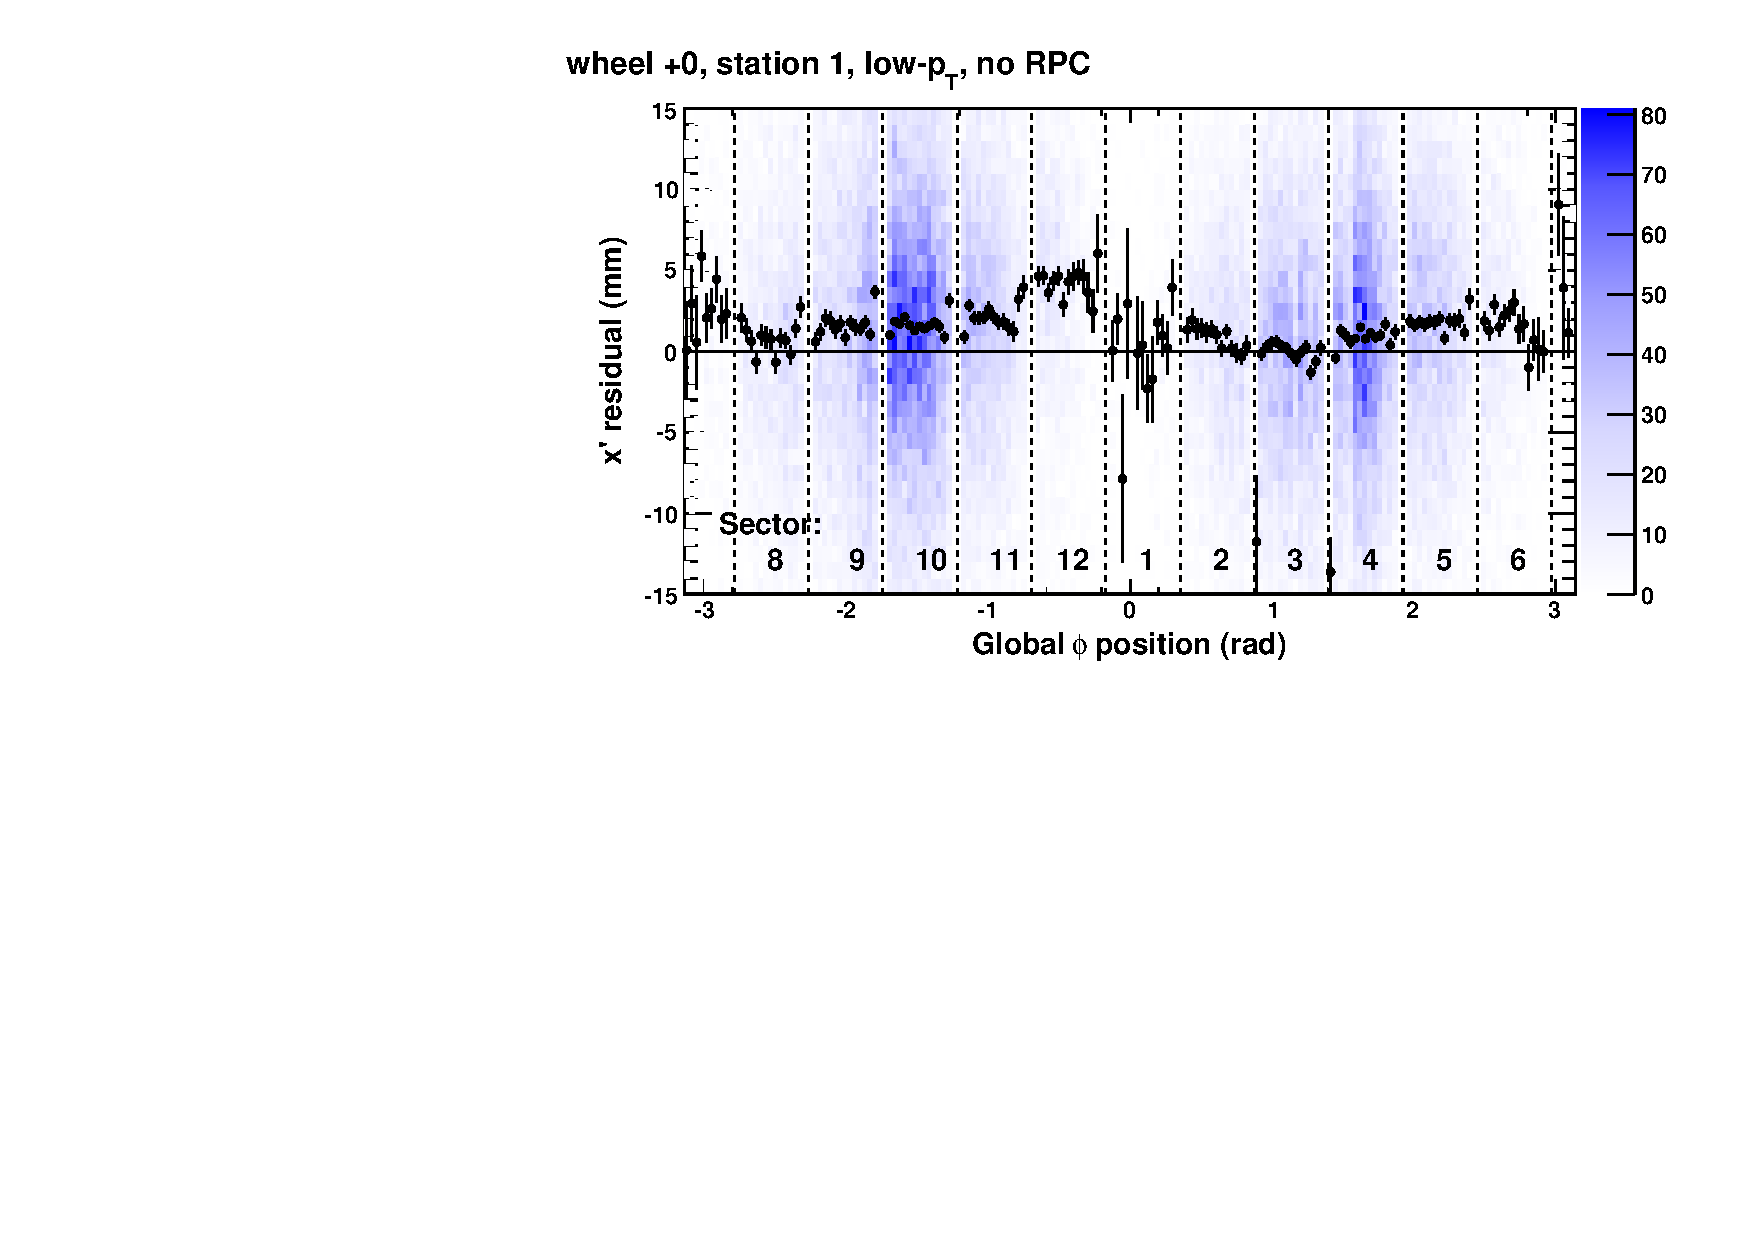
\includegraphics[width=0.9\linewidth]{sawtoothexample_x_low_norpc.pdf}
\end{columns}

\begin{columns}
\column{0.49\linewidth}
\hfill 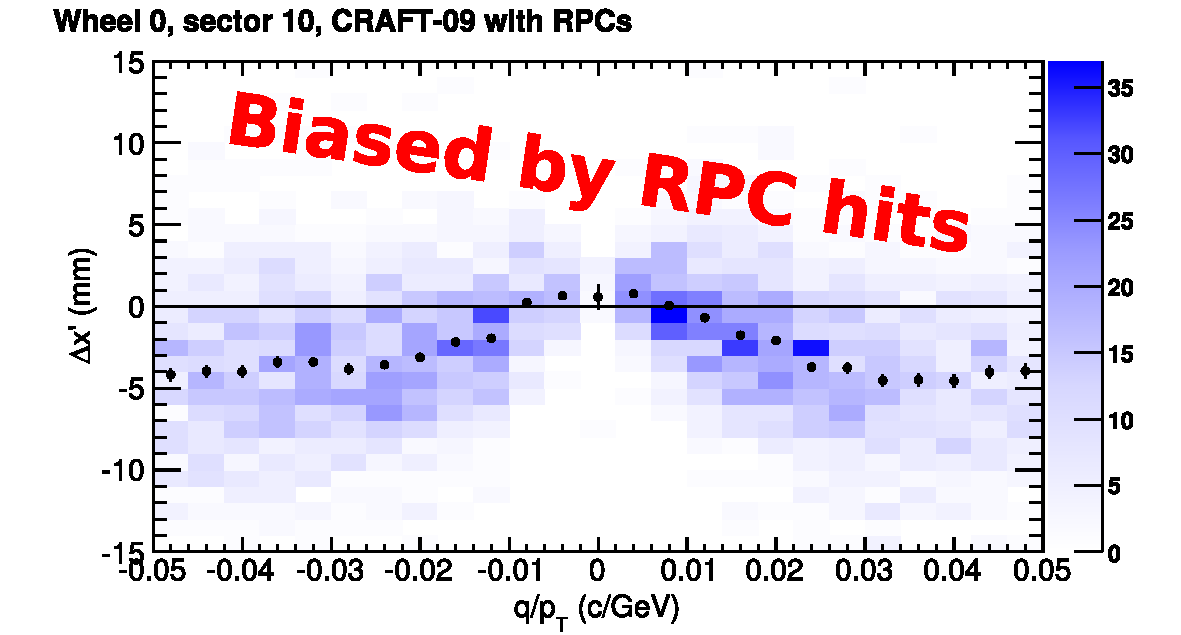
\includegraphics[width=0.9\linewidth]{globaldistort_withRPC.pdf}

\column{0.02\linewidth}
$\mathbf{\to}$

\column{0.49\linewidth}
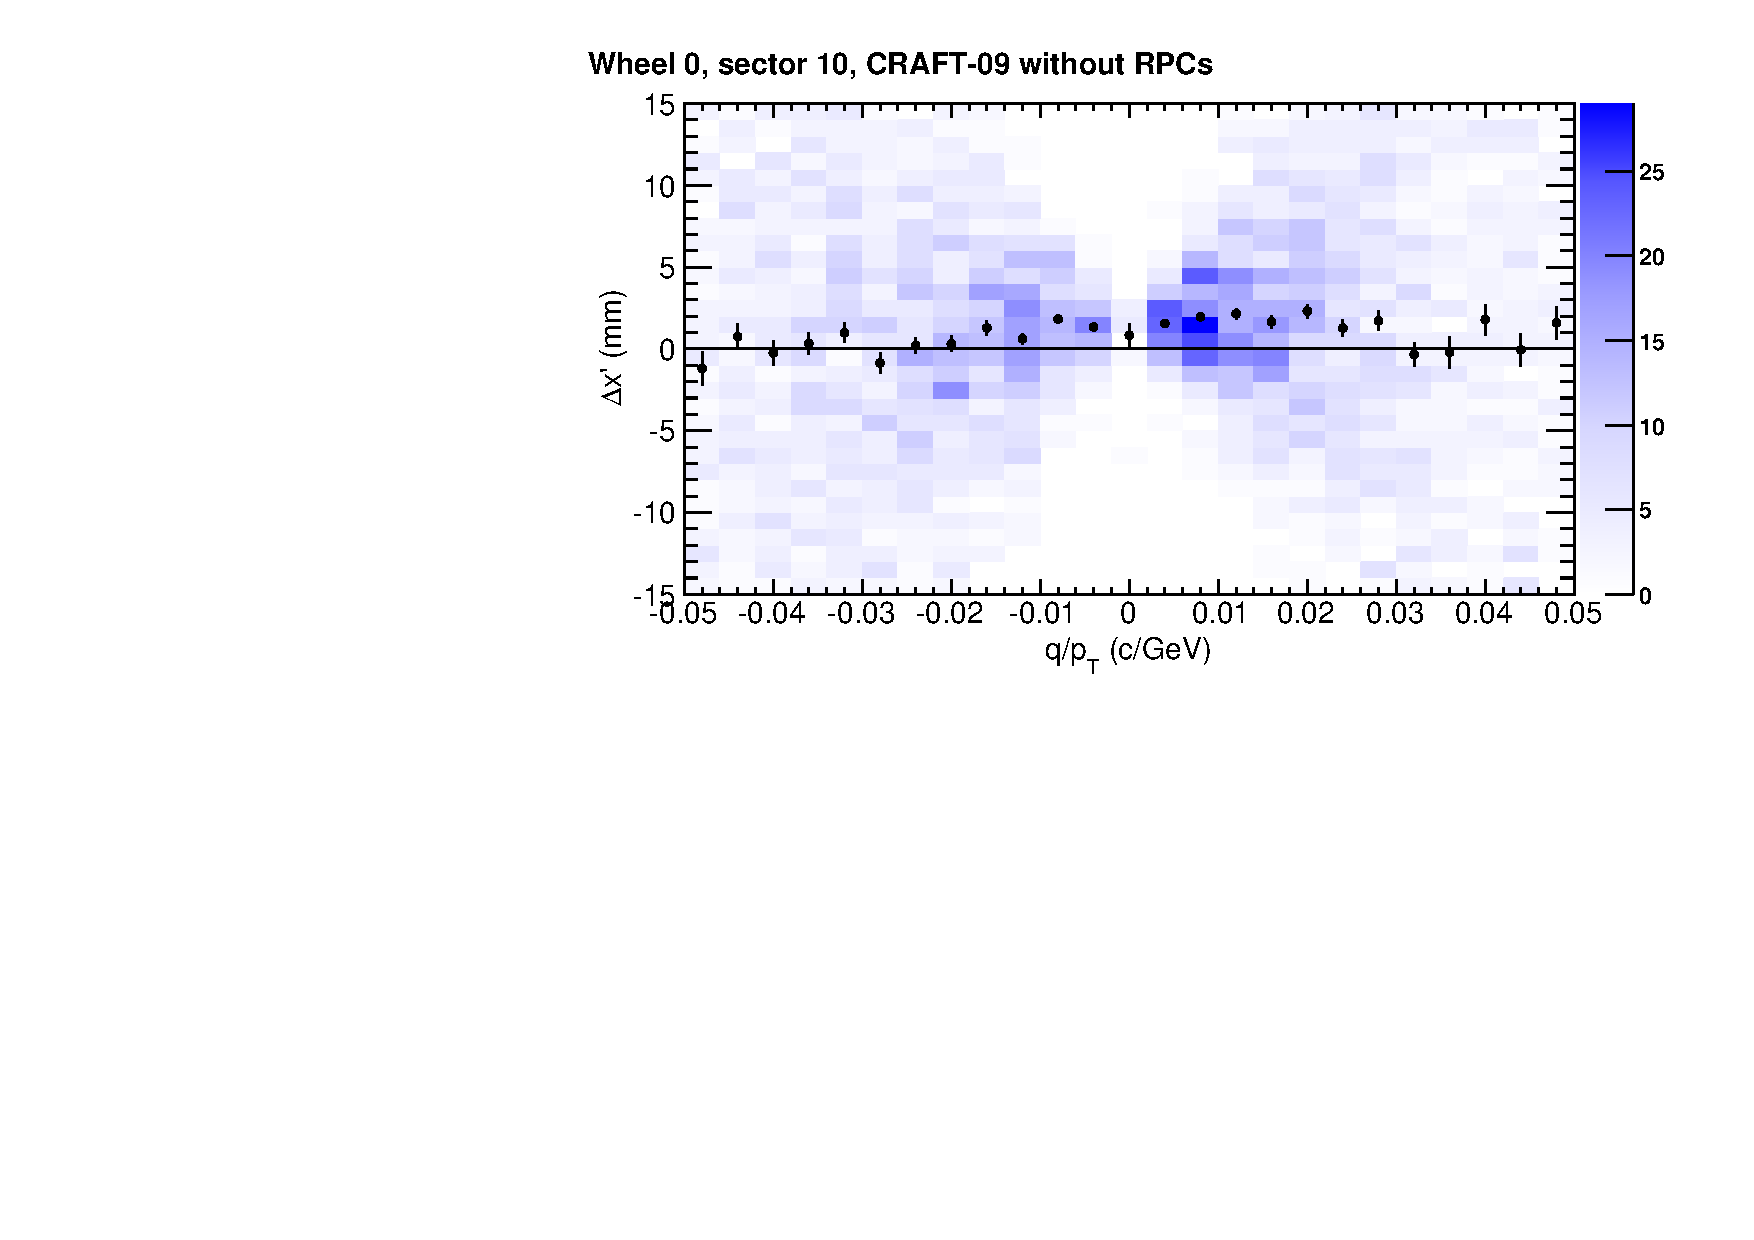
\includegraphics[width=0.9\linewidth]{globaldistort_noRPC.pdf}
\end{columns}

\vspace{0.2 cm}
\hspace{-0.83 cm} \textcolor{darkblue}{\Large Outline}

\begin{itemize}
\item Recomputed muon alignment without this bias
\item Redo tracker weak mode study
\item We confirm the momentum scale error that Pablo sees \mbox{in CRAFT-10\hspace{-1 cm}} \\ (and we do {\it not} see it in CRAFT-09)
\end{itemize}
\end{frame}

\begin{frame}
\frametitle{How did this happen?}
\begin{description}\setlength{\itemsep}{0.3 cm}
\item[Feb 2007:] Discovered that RPC hits were biasing the alignment track refits (should have muon APE $\to \infty$, can't set RPC APEs)

\item[Aug 2007:] ``RefitRPCHits'' switch integrated into CMSSW; track
  refits are unbiased by RPC hits when set to ``False''

\item[$\begin{array}{c} \mbox{sometime} \\ \mbox{before} \\ \mbox{CRAFT-08:} \end{array}$] Made the following mistake in Python configuration file:

TrackRefitter.RefitRPCHits = False

\hfill \textcolor{red}{\it \# CMSSW doesn't complain; uses default (True)}

\vspace{0.25 cm}
instead of

\vspace{0.25 cm}
\textcolor{gray}{TrackRefitter}.TrackTransformer.\textcolor{gray}{RefitRPCHits = False}

\hfill \textcolor{red}{\it \# what we want}
\end{description}

\textcolor{darkblue}{RPC hits were being included in track refits because of a typo}
\end{frame}

\begin{frame}
\frametitle{Controlling the problem}

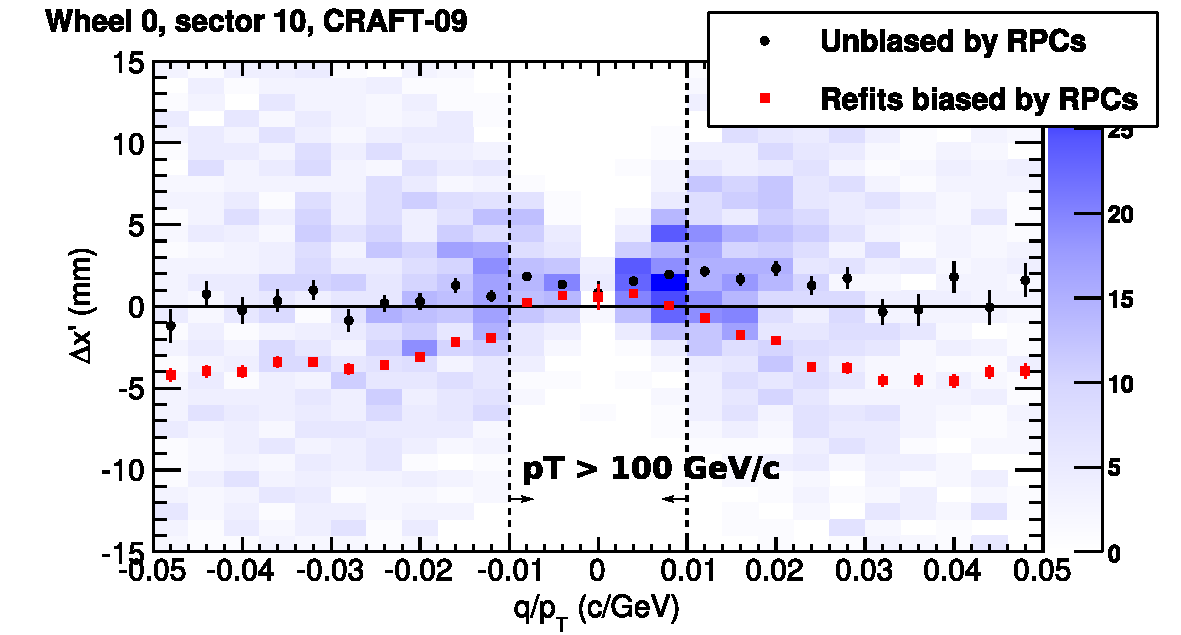
\includegraphics[width=0.9\linewidth]{globaldistort_compare.pdf}

\begin{itemize}
\item We saw that we had a problem, but couldn't identify the source
\item We knew from other studies that the high-momentum tracks were the most trustworthy
\item Applied a $p_T > 100$~GeV/$c$ cut to limit the bias
\begin{itemize}
\item now that it is understood, we can loosen this cut
\end{itemize}
\end{itemize}
\end{frame}

\begin{frame}
\frametitle{Re-alignment without RPC bias}

\begin{itemize}
\item Below: differences between aligned parameters without RPC-hit bias and aligned parameters with the bias
\end{itemize}

\begin{columns}
\column{0.7\linewidth}
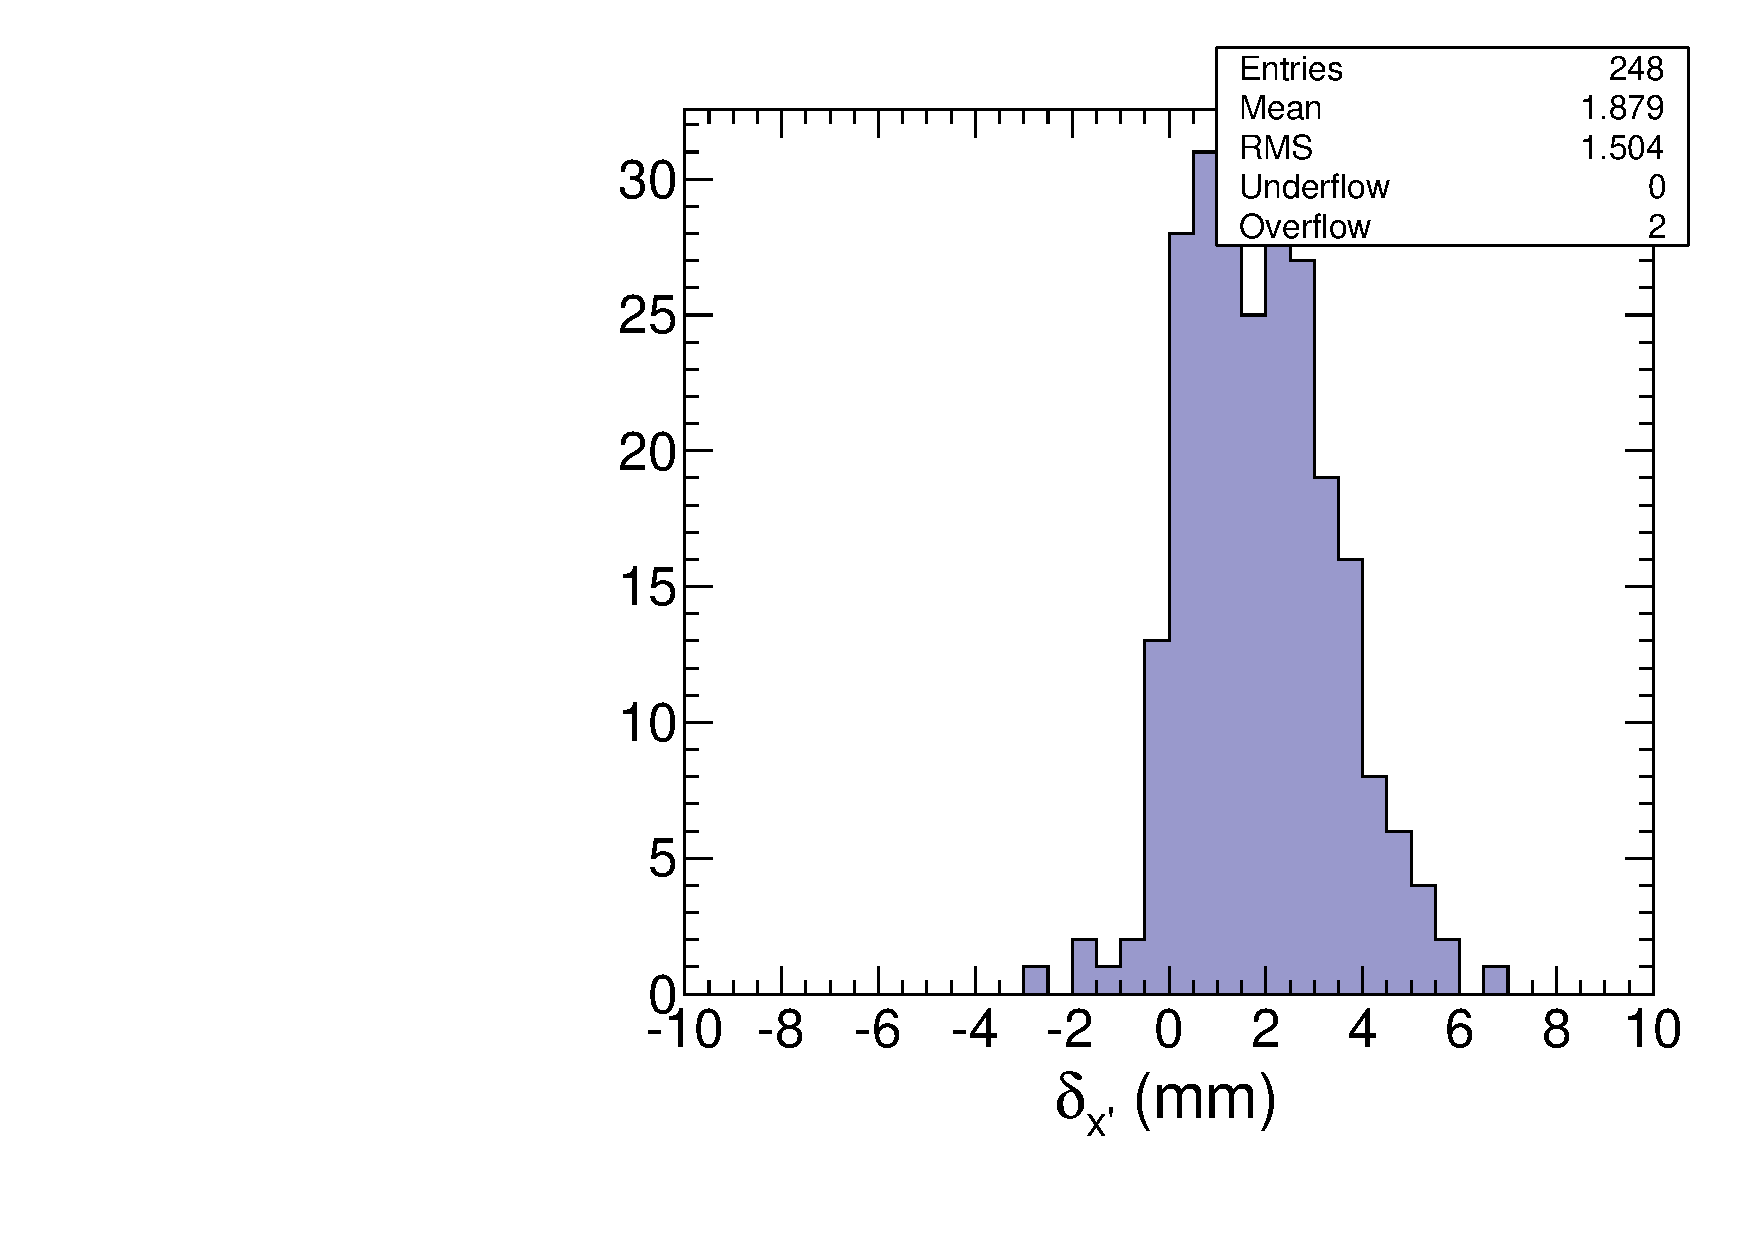
\includegraphics[width=0.5\linewidth]{01_deltax_with_and_without_RPC.pdf}
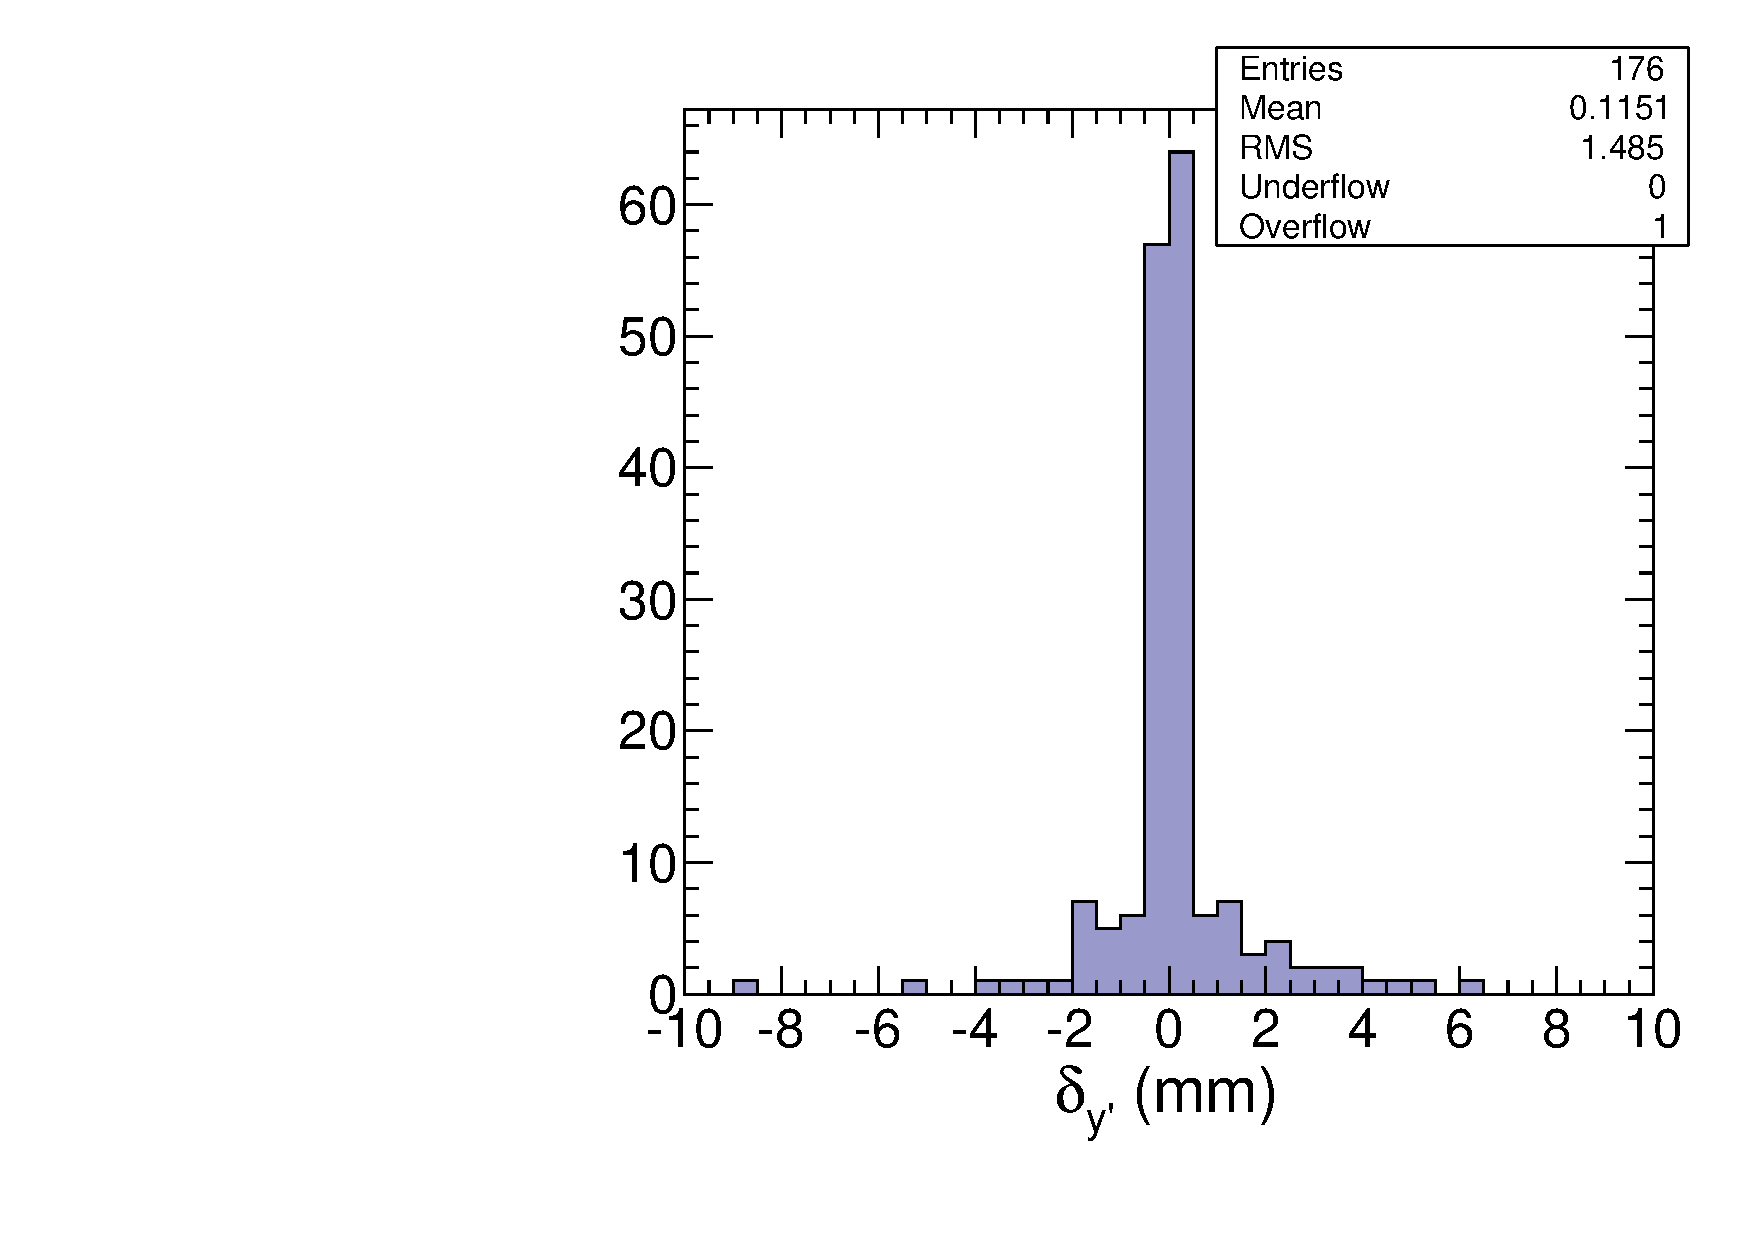
\includegraphics[width=0.5\linewidth]{02_deltay_with_and_without_RPC.pdf}

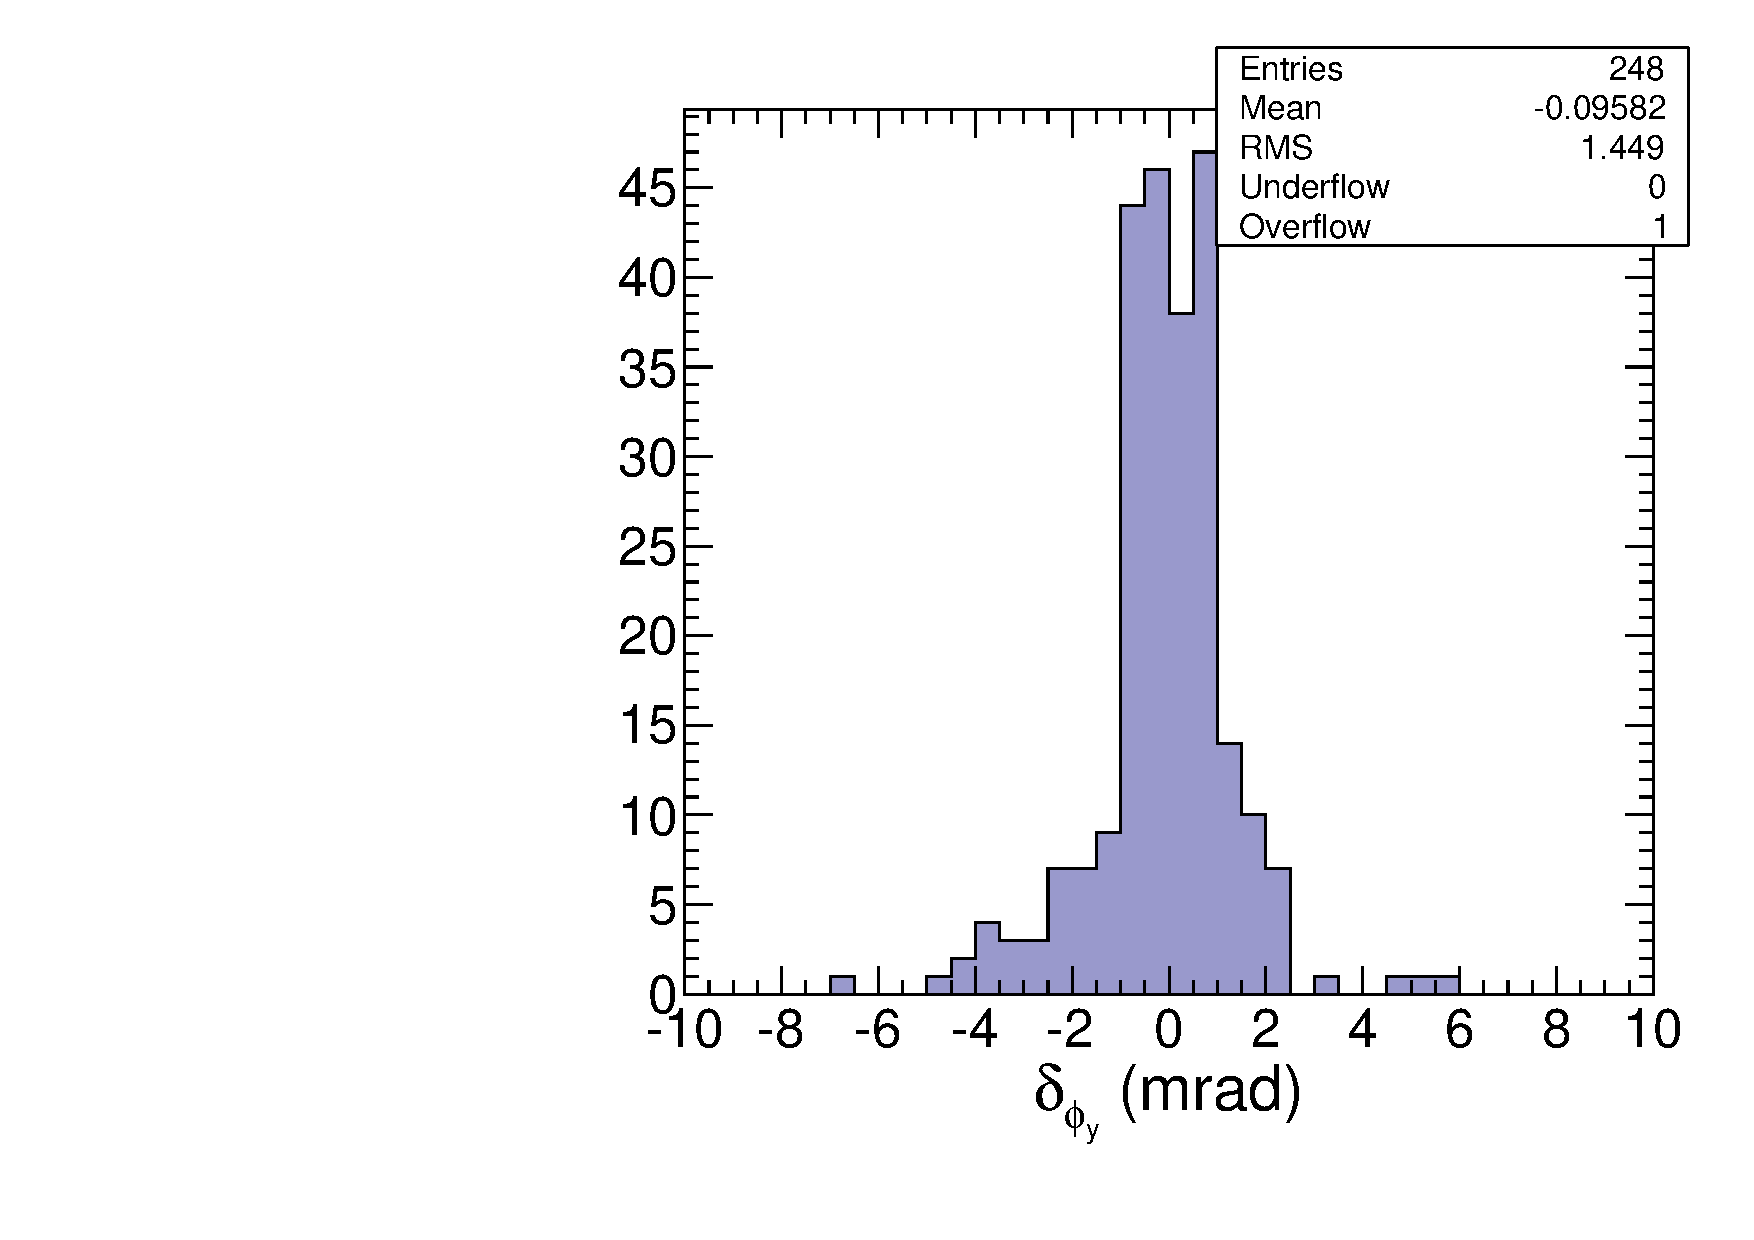
\includegraphics[width=0.5\linewidth]{03_deltaphiy_with_and_without_RPC.pdf}
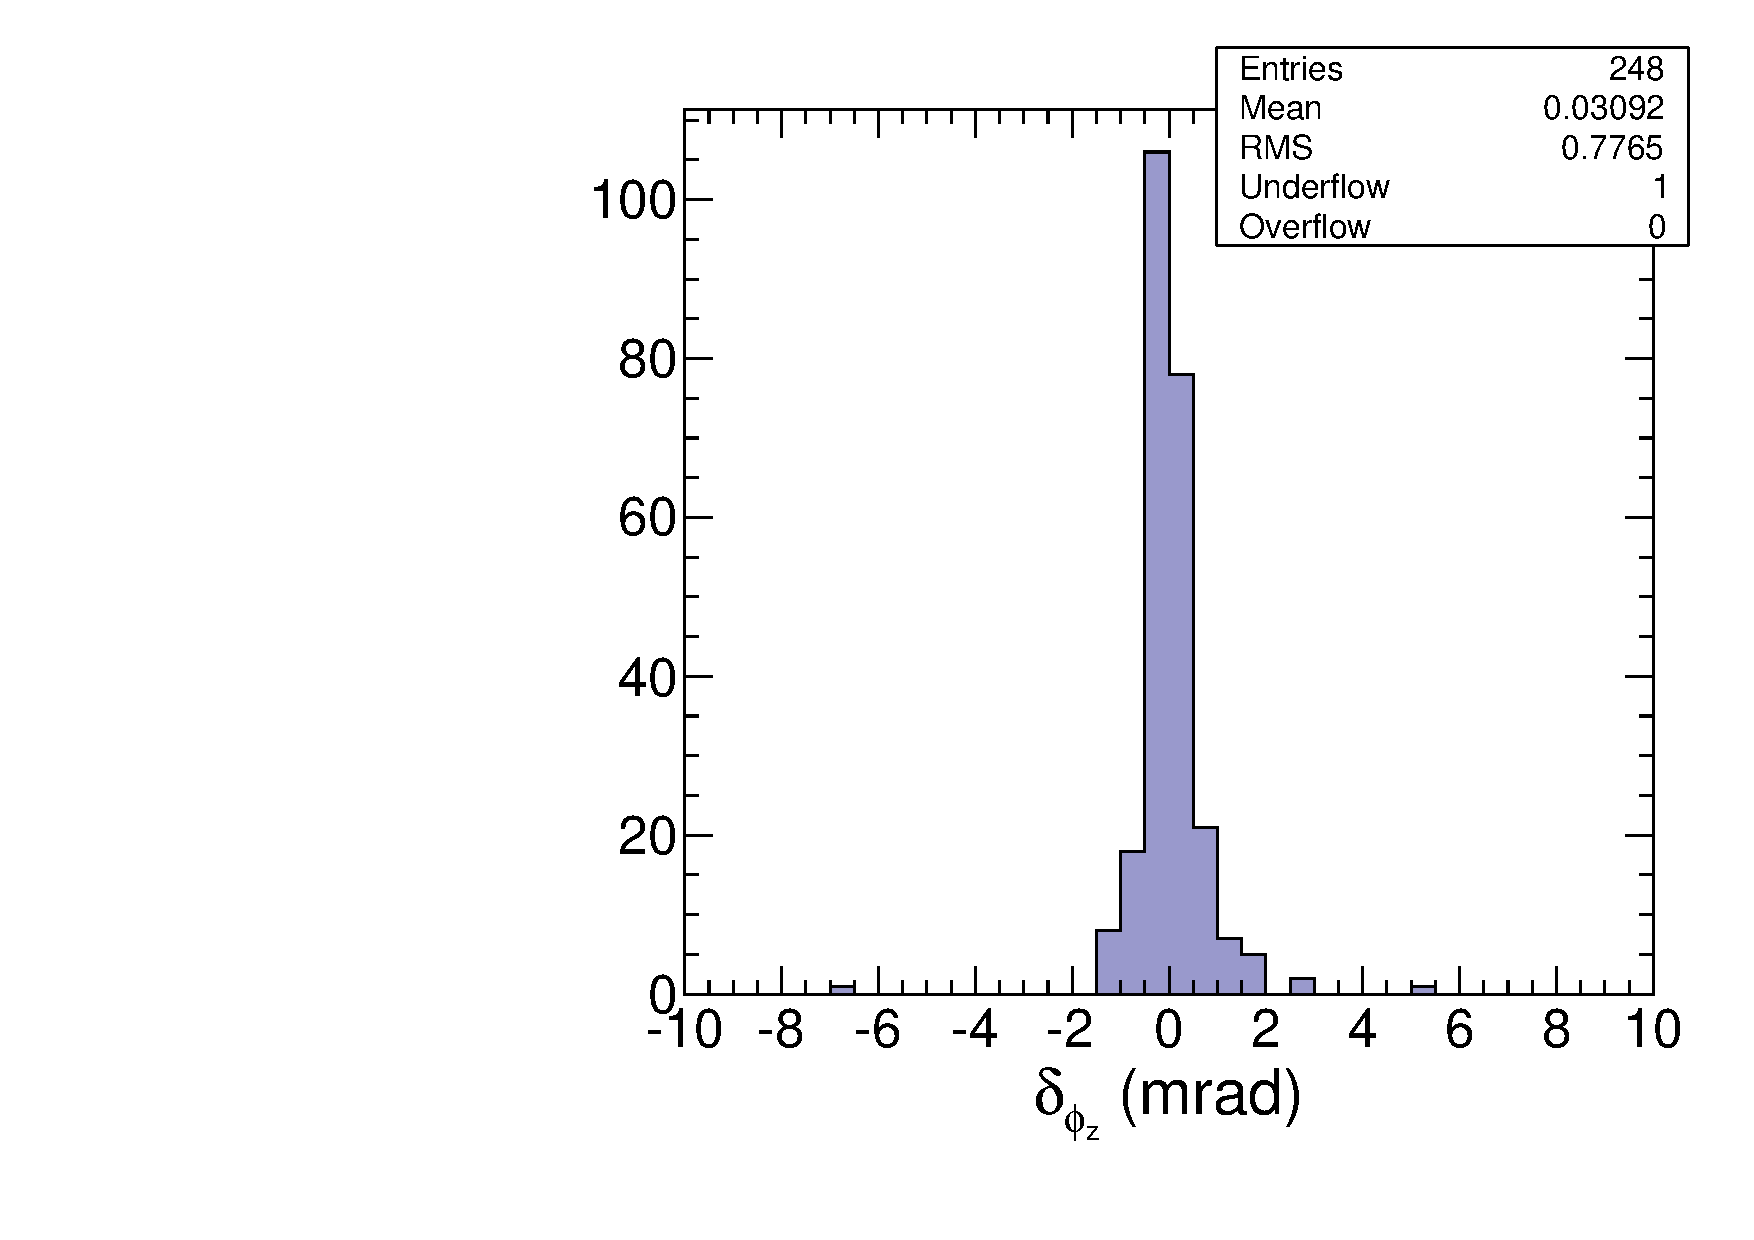
\includegraphics[width=0.5\linewidth]{04_deltaphiz_with_and_without_RPC.pdf}

\column{0.3\linewidth}
This will be a significant correction!

\begin{itemize}
\item Effective rotation of about 0.3~mrad around the beamline ($\delta_{x'}$)
\item RMS spread of 1.5~mm
\item Would have been 5~mm if not for the 100~GeV/$c$ cut
\end{itemize}

\hfill \textcolor{darkblue}{\scriptsize CRAFT-10}
\end{columns}
\end{frame}

\begin{frame}
\frametitle{Agreement with cross-alignment}

\begin{itemize}
\item Sasha Spiridonov developed a method to align the muon
  system relative to tracker by comparing tracker tracks \mbox{with standAloneMuons\hspace{-1 cm}}
\begin{itemize}
\item standAloneMuons are insensitive to RPC hits
\end{itemize}
\item Without RPC bias, Reference-Target now agrees with this method
\end{itemize}

\only<1>{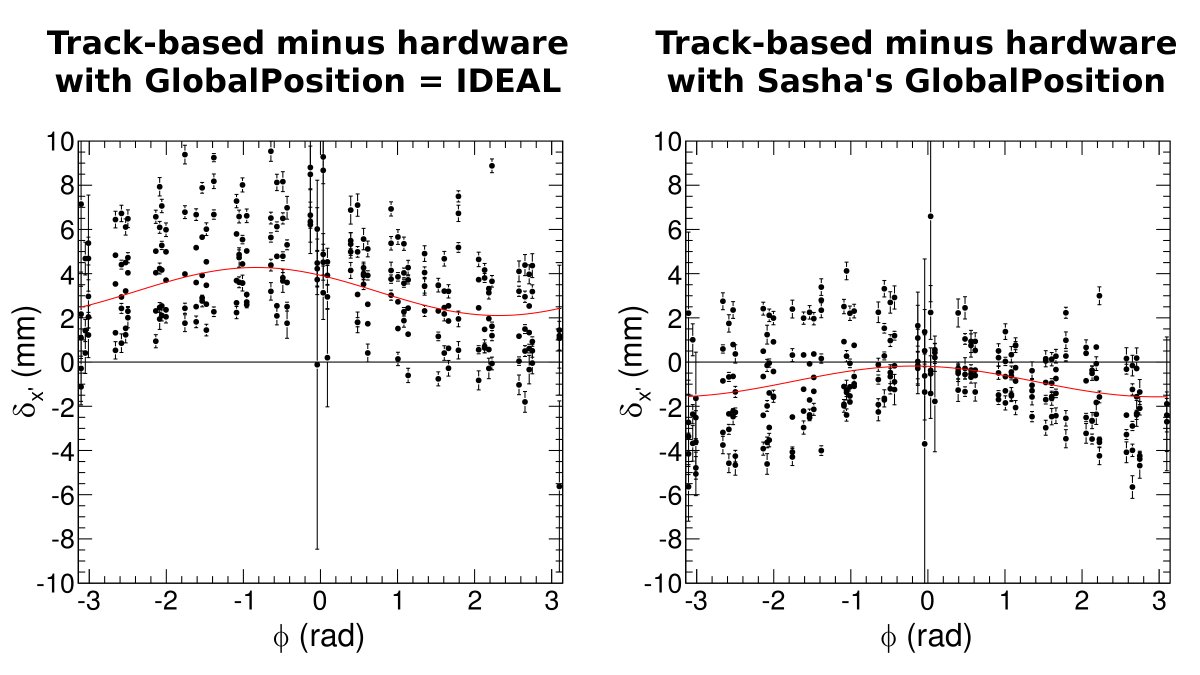
\includegraphics[width=\linewidth]{deltax_track-based_minus_hardware.png}}
\only<2>{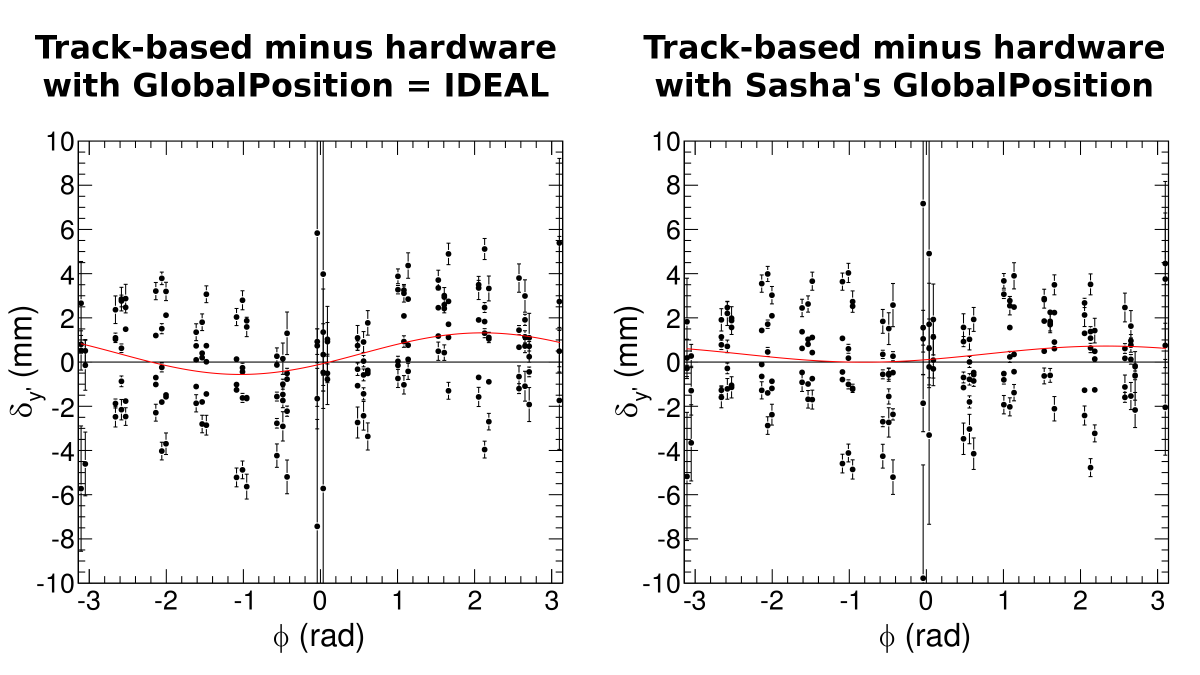
\includegraphics[width=\linewidth]{deltay_track-based_minus_hardware.png}}
\end{frame}

%% \begin{frame}
%% \frametitle{Sawtooth effect in endcap (new)}

%% \vspace{-0.25 cm}
%% \begin{columns}
%% \column{0.5\linewidth}
%% \begin{itemize}
%% \item Aysen began studying CSC residuals from collisions globalMuons just last week
%% \item Saw strong sawtooth in ME1/2, but not elsewhere; \\ eliminated by excluding RPC hits from refits
%% \end{itemize}

%% \column{0.5\linewidth}
%% 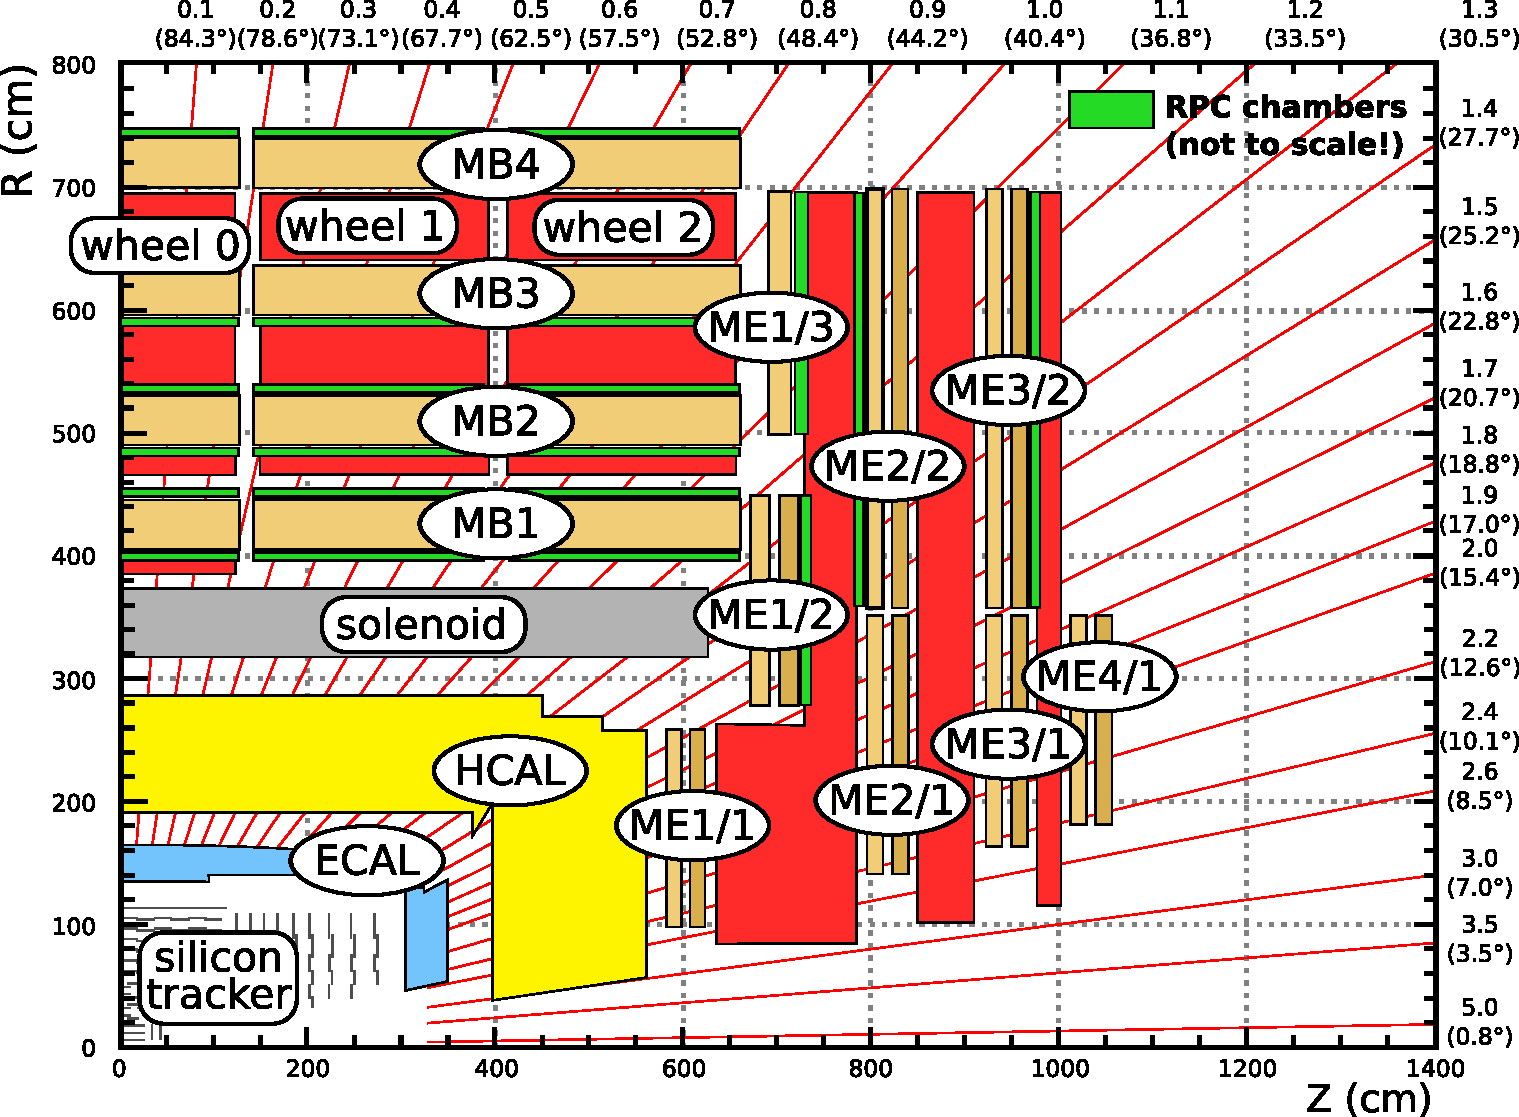
\includegraphics[width=\linewidth]{muon_system_withRPC.pdf}
%% \end{columns}

%% \vspace{0.25 cm}
%% \begin{columns}
%% \column{0.5\linewidth}
%% track refits biased by RPC hits

%% 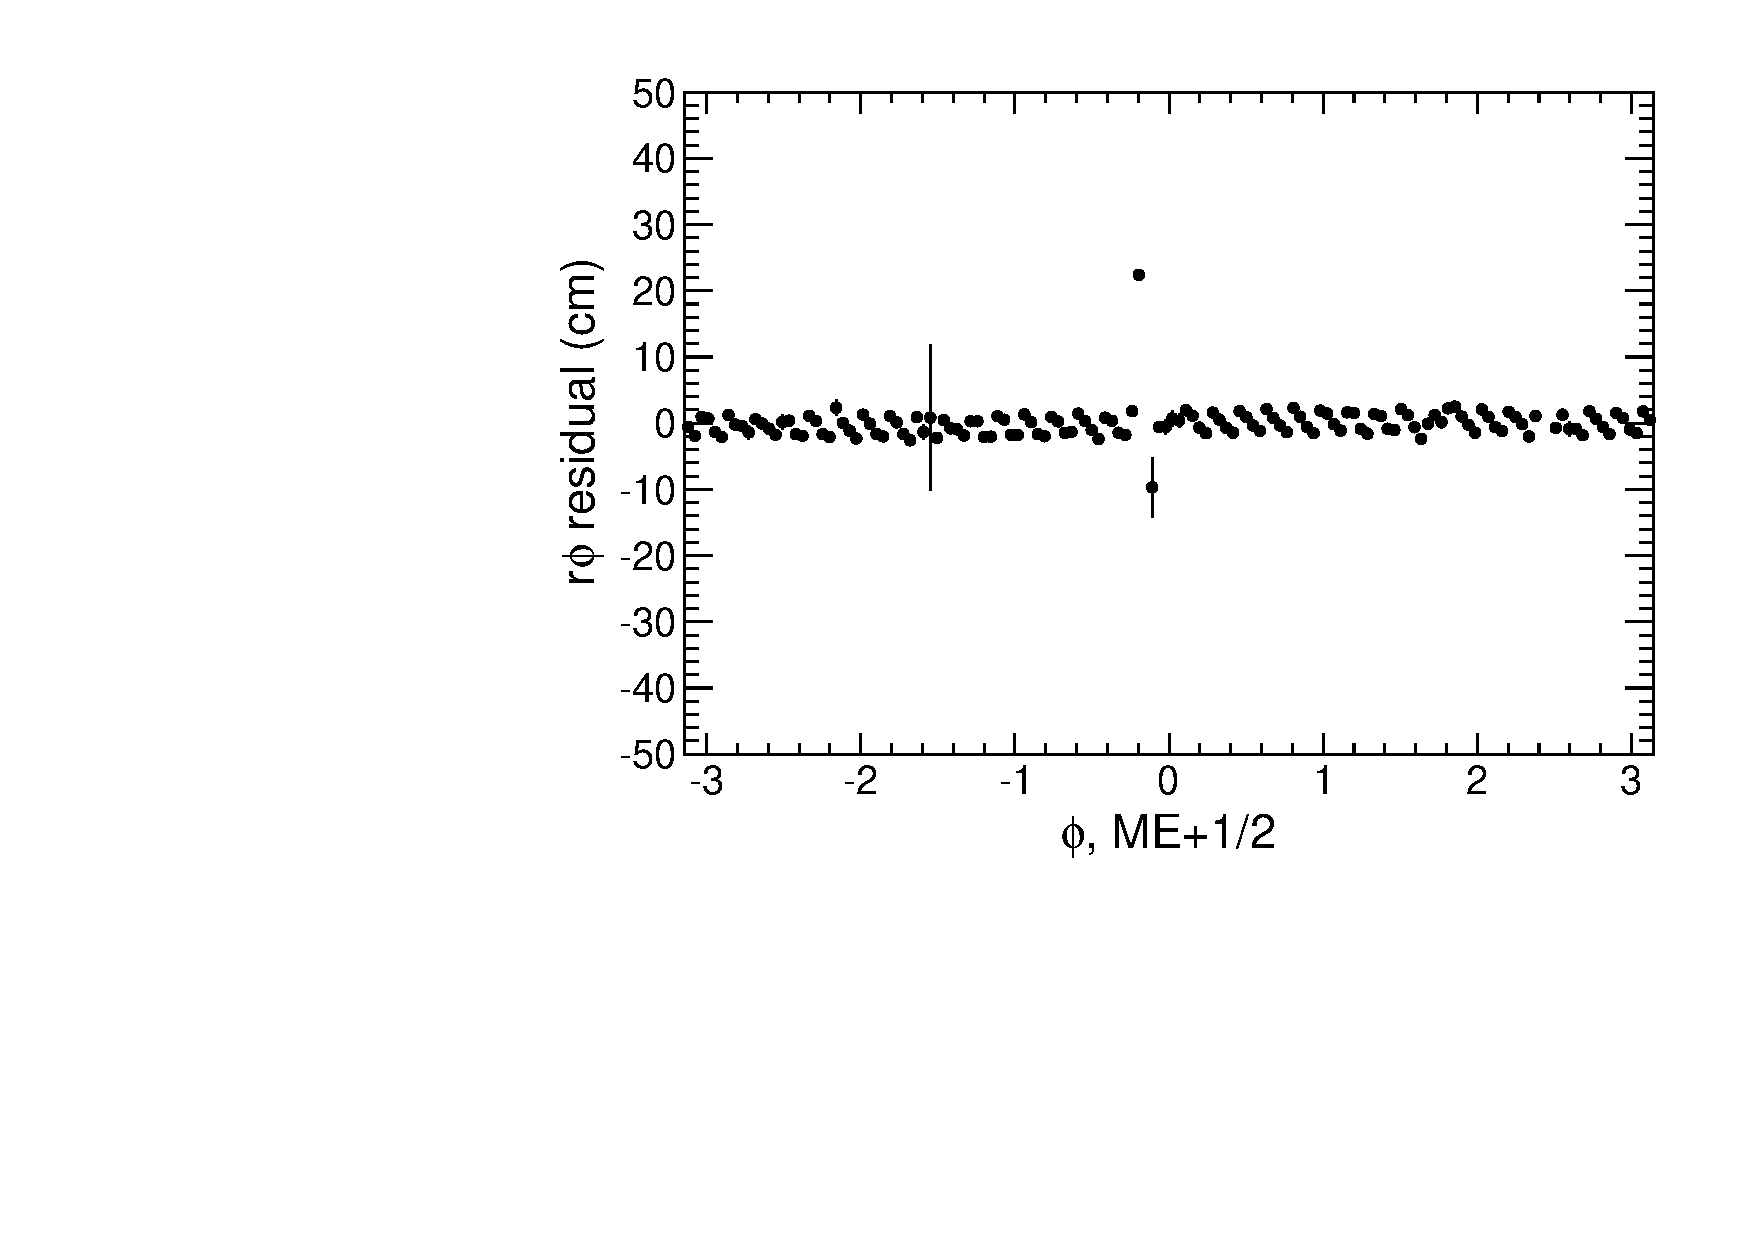
\includegraphics[width=\linewidth]{deltax_phi_prof_mep12_refitRPC.pdf}

%% \column{0.5\linewidth}
%% unbiased track refits

%% 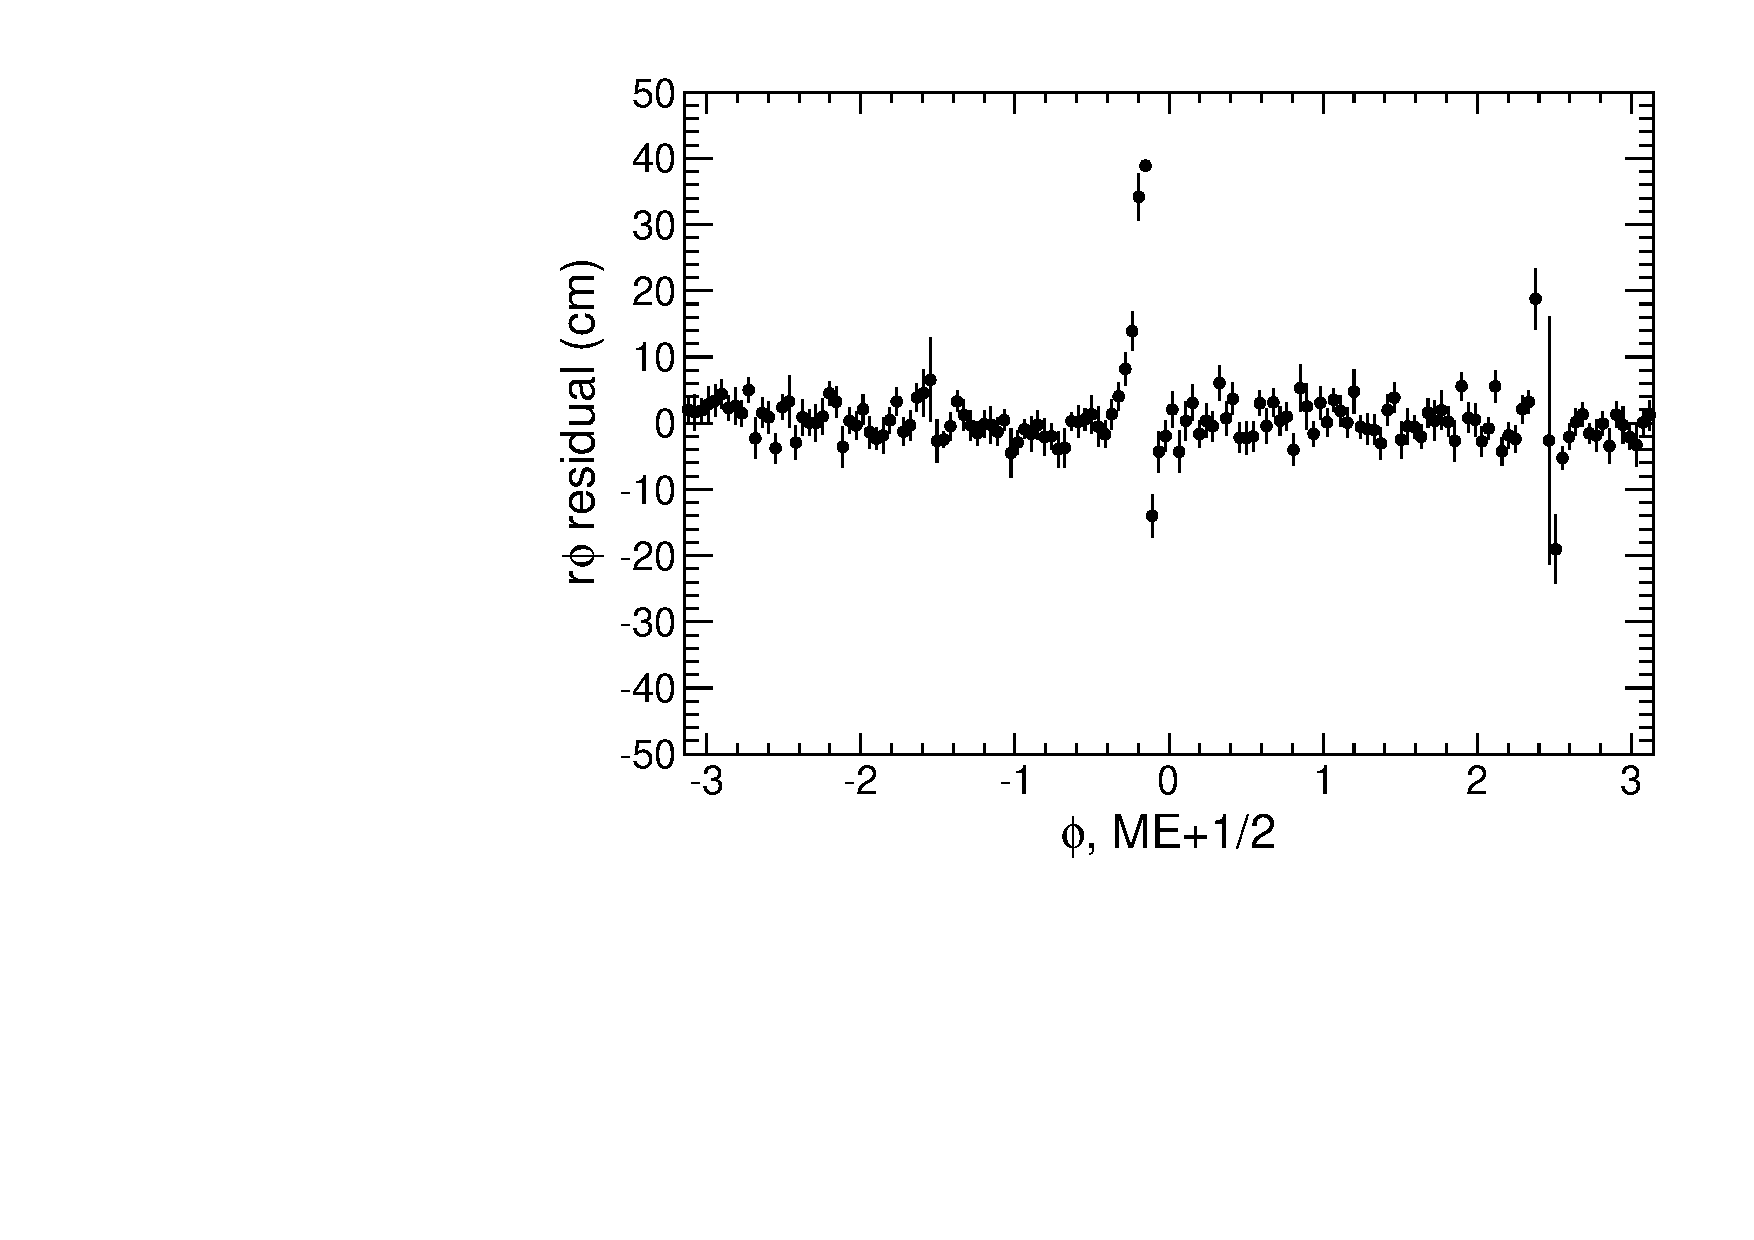
\includegraphics[width=\linewidth]{deltax_phi_prof_mep12_norefitRPC.pdf}
%% \end{columns}

%% \vspace{-1.25 cm}
%% \hfill \textcolor{darkblue}{\scriptsize 2010 collisions data}
%% \end{frame}

\begin{frame}
\frametitle{Tracker weak mode study}

\begin{columns}
\column{0.5\linewidth}
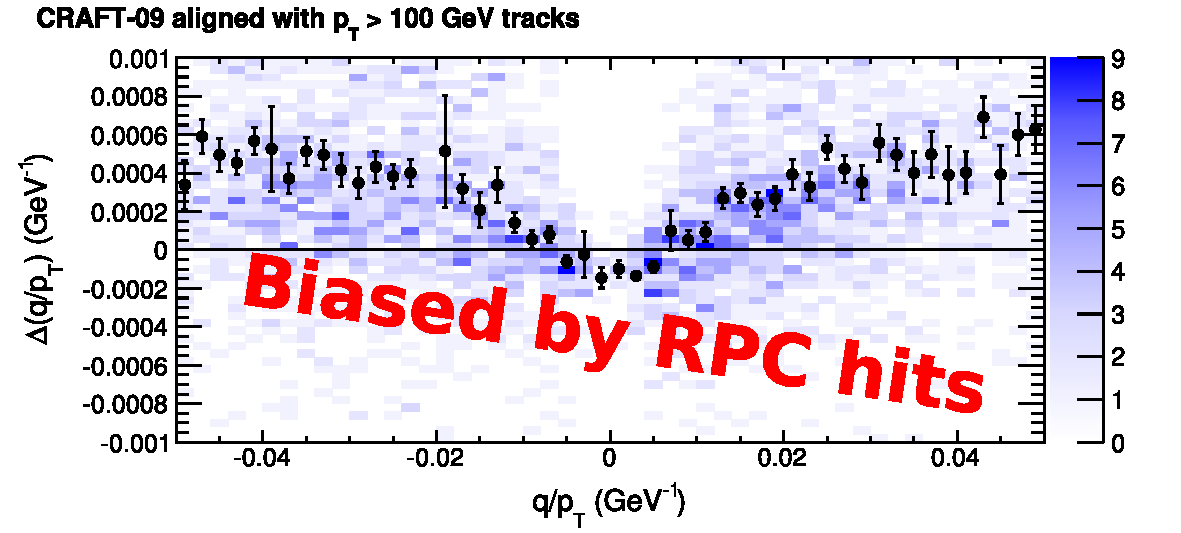
\includegraphics[width=\linewidth]{curvature_real.pdf}

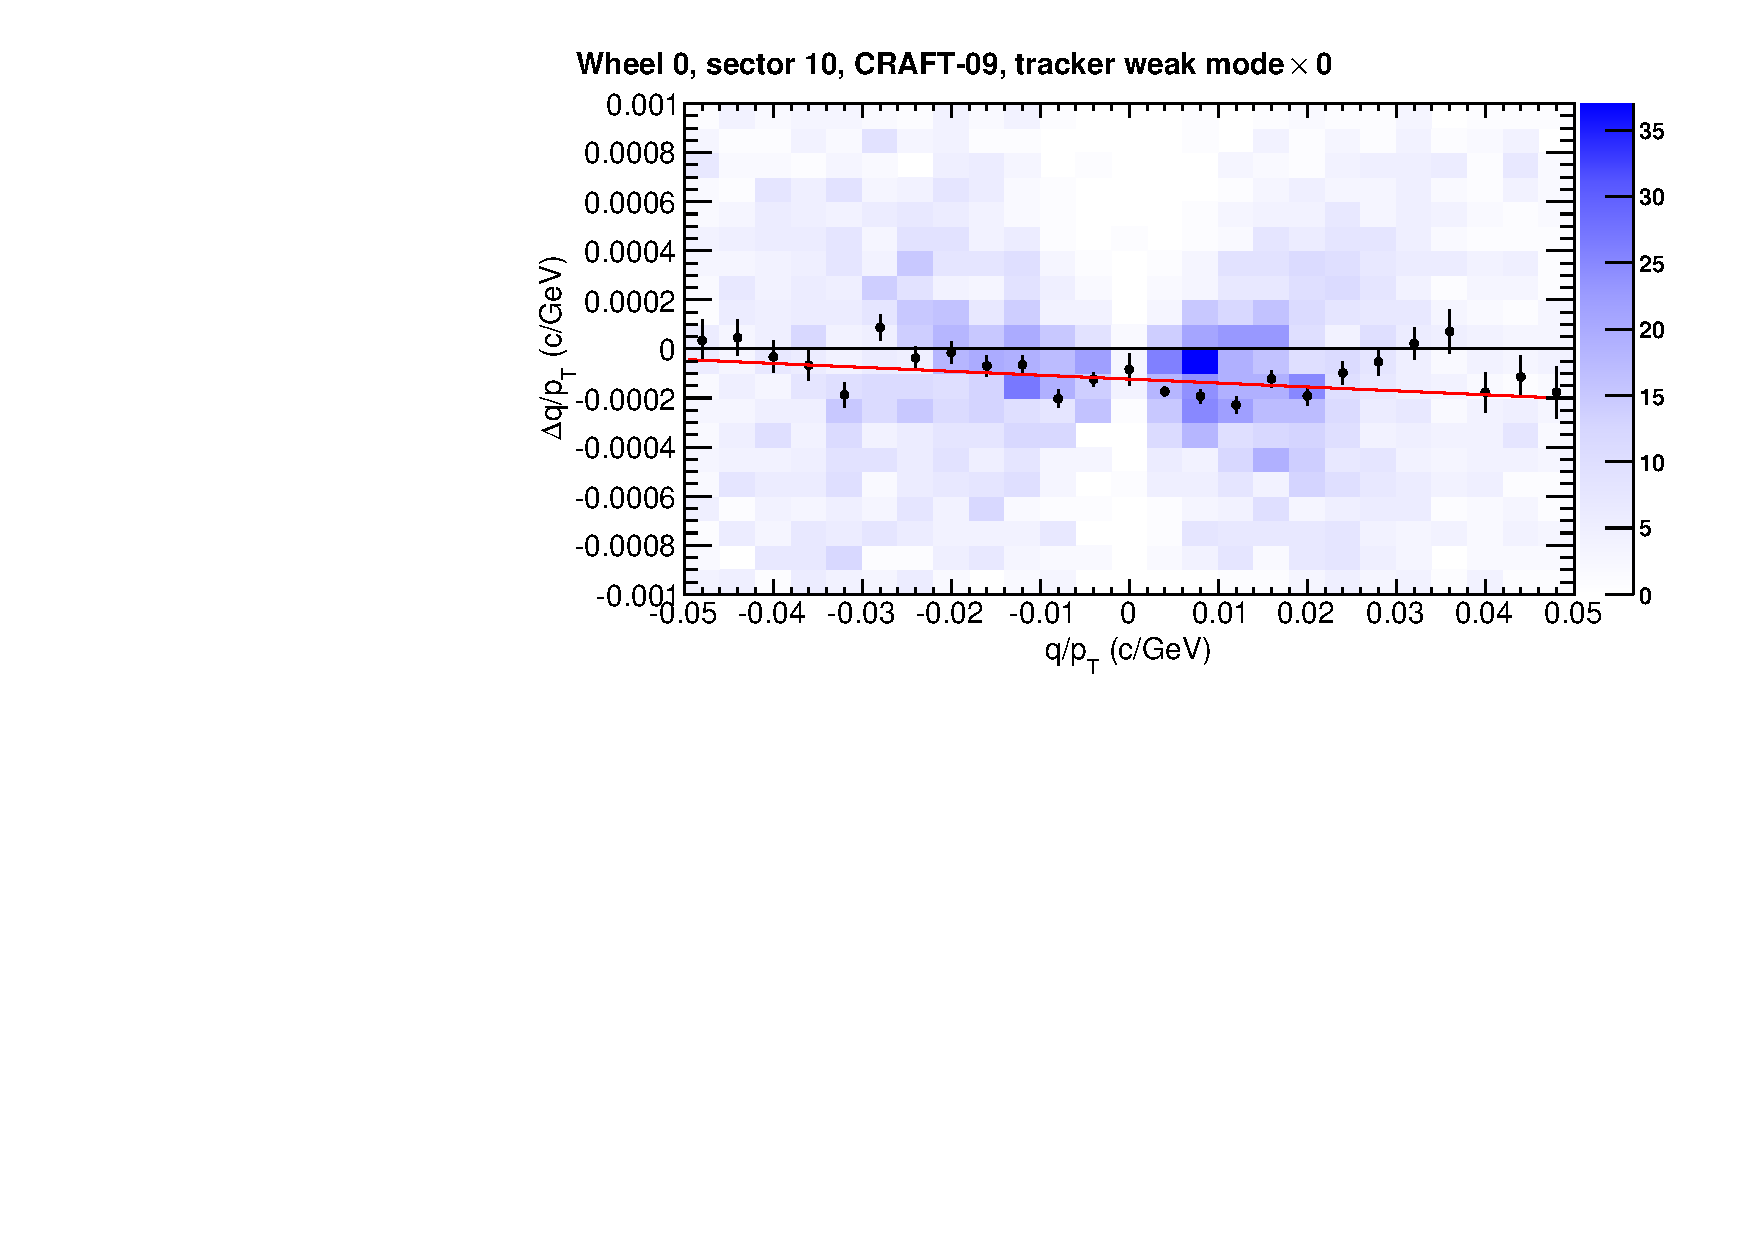
\includegraphics[width=\linewidth]{weakmode_times0.pdf}

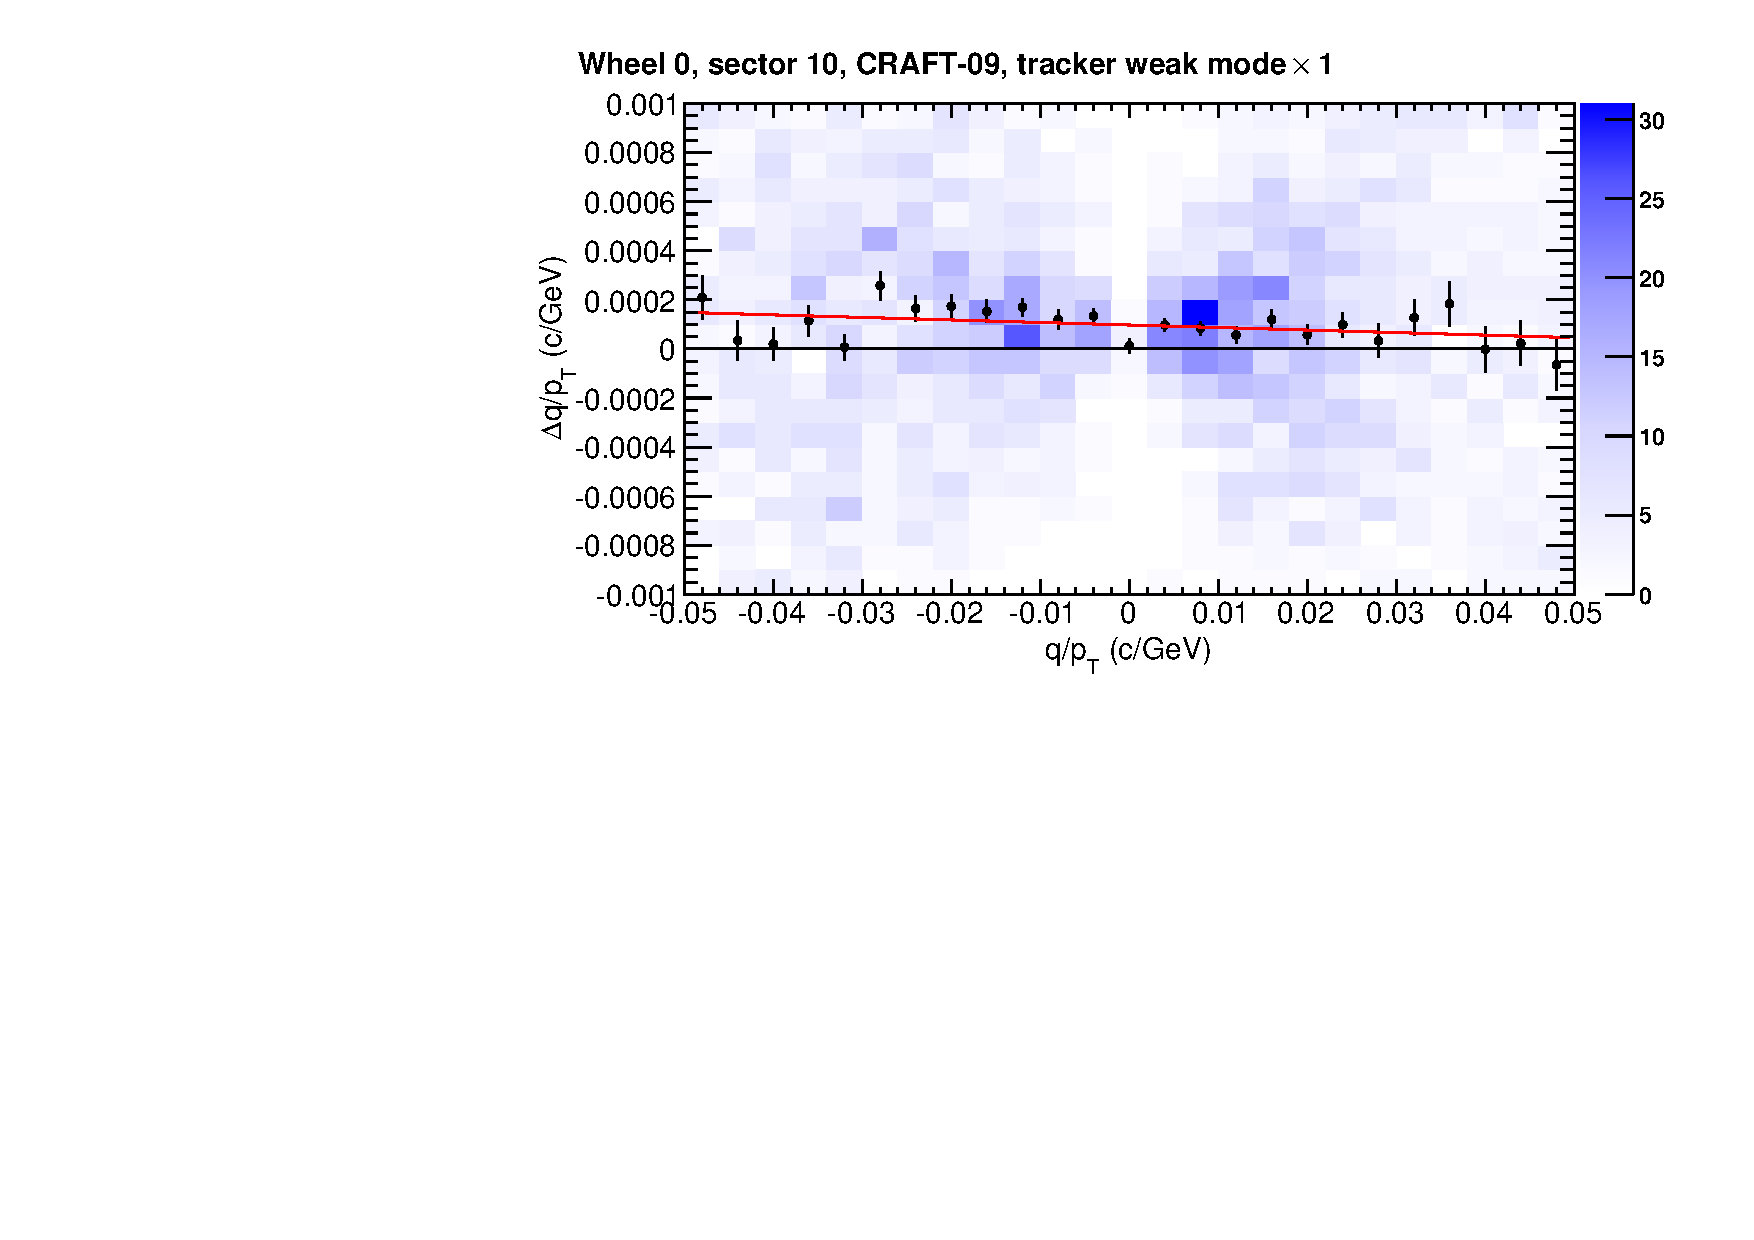
\includegraphics[width=\linewidth]{weakmode_times1.pdf}

\vspace{-1 cm}
\hfill \textcolor{darkblue}{\scriptsize \mbox{CRAFT-09\hspace{-1.2 cm}}}

\vspace{0.5 cm}

\column{0.5\linewidth}

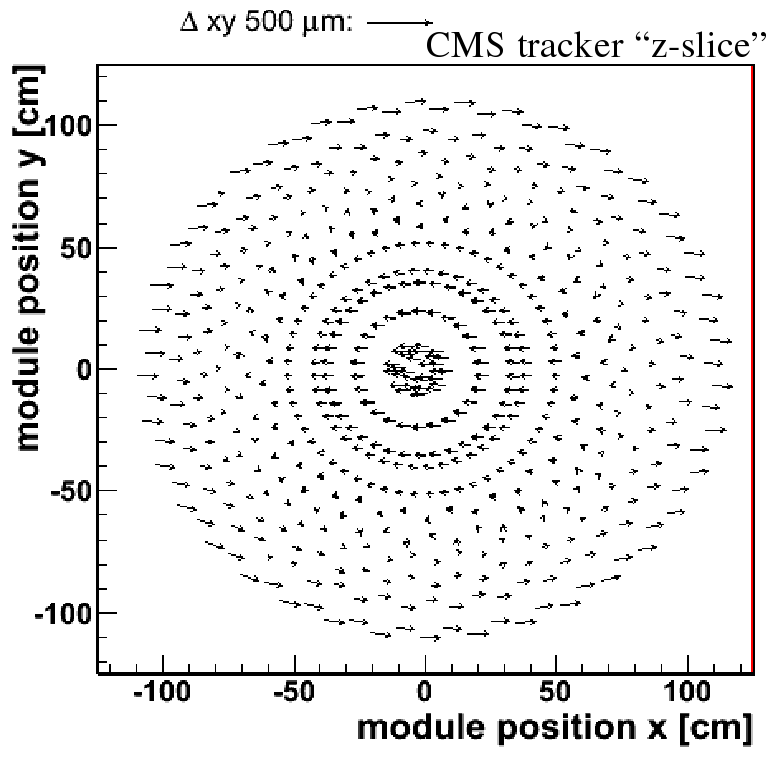
\includegraphics[width=0.5\linewidth]{stoye_deformation.png}
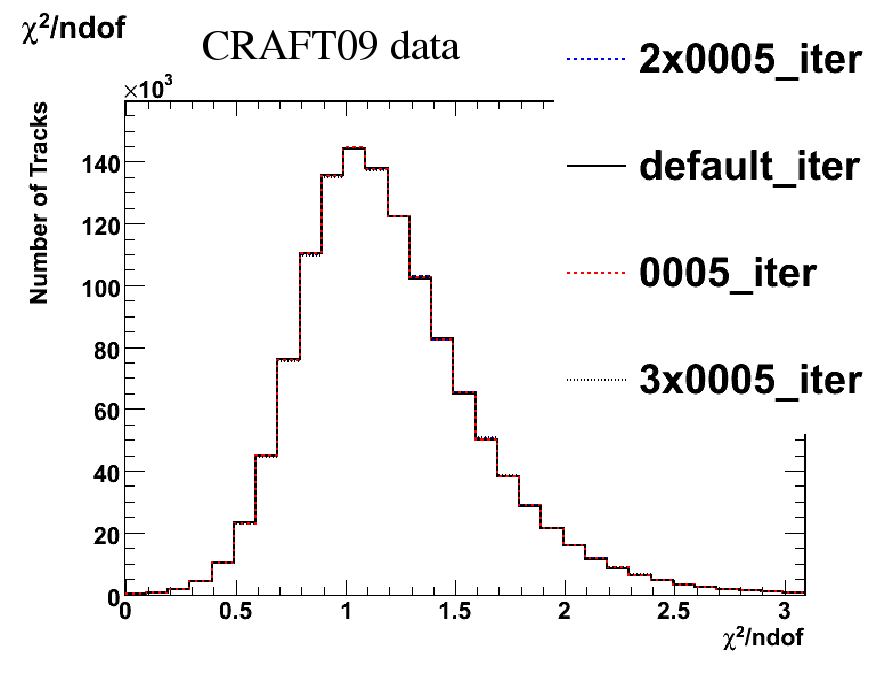
\includegraphics[width=0.5\linewidth]{chi2_invariance.png}

\begin{itemize}
\item Apply Millepede-generated mode to correctly-calculated muon residuals

\item No distortion with ``100~GeV/$c$ characteristic scale'': that was the RPCs

\item Only a constant \mbox{shift in $\Delta(q/p_T)$\hspace{-1 cm}}

\item Can't distinguish tracker weak mode from muon alignment (but limits on tracker weak modes imply $\sigma_x \lesssim 0.25$~mm)
\end{itemize}
\end{columns}
\end{frame}

\begin{frame}
\frametitle{Reminder of $\vec{B}$-sensitive residuals}

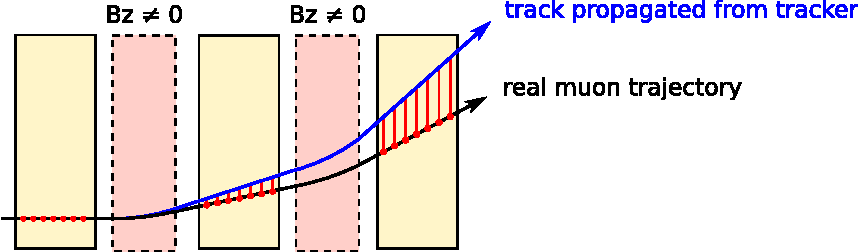
\includegraphics[width=0.75\linewidth]{paths.pdf}

\vspace{-0.75 cm}
\hfill \begin{minipage}{0.55\linewidth}
Position residuals: more sensitive to a momentum scale problem, but harder to interpret
\end{minipage}

\hfill 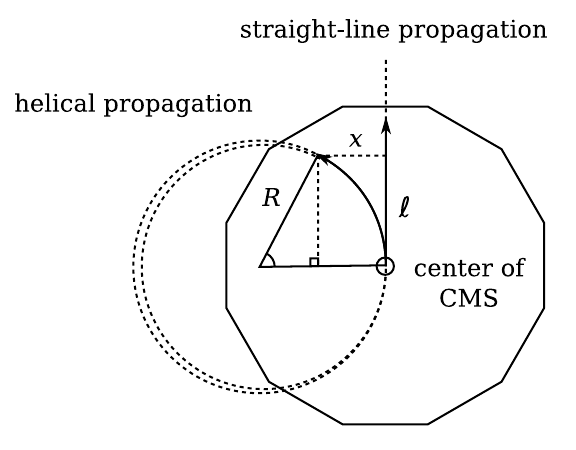
\includegraphics[width=0.3\linewidth]{bfield_derivation.png}

\vspace{-1.5 cm}
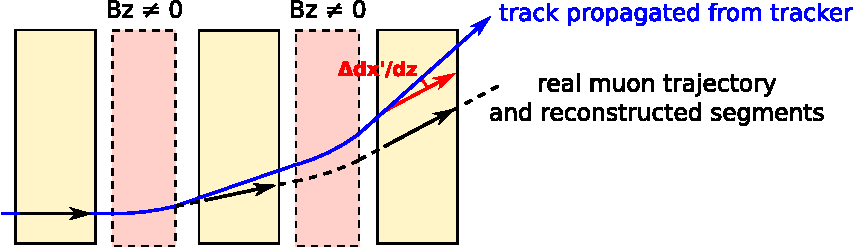
\includegraphics[width=0.75\linewidth]{paths2.pdf}

\vspace{-0.75 cm}
\hfill \begin{minipage}{0.55\linewidth}
Angle resids: $\displaystyle \frac{\Delta dx'/dz}{q/p_T} = \int \frac{\Delta B_z(\ell)}{\mbox{330~cm}} d\ell$

\vspace{0.2 cm}
{\scriptsize $\Delta dx'/dz$ in rad, $q/p_T$ in $c$/GeV, $\Delta B_z$ in Tesla}
\end{minipage}

\vspace{0.5 cm} Note: sign of inferred $\Delta B_z$ is reversed in the
top of CMS (sectors 1--6), where the muons' momentum vector points
toward the beamline.
\end{frame}

\begin{frame}
\frametitle{Position residuals}

Momentum scale error introduced this year \mbox{(same sign in top and bottom)\hspace{-1 cm}}

\vspace{-0.5 cm}
\begin{tabular}{p{0.45\linewidth} p{0.45\linewidth}}
\begin{center} \large \textcolor{darkblue}{CRAFT-09} \end{center} & \begin{center} \large \textcolor{darkblue}{CRAFT-10} \end{center} \\
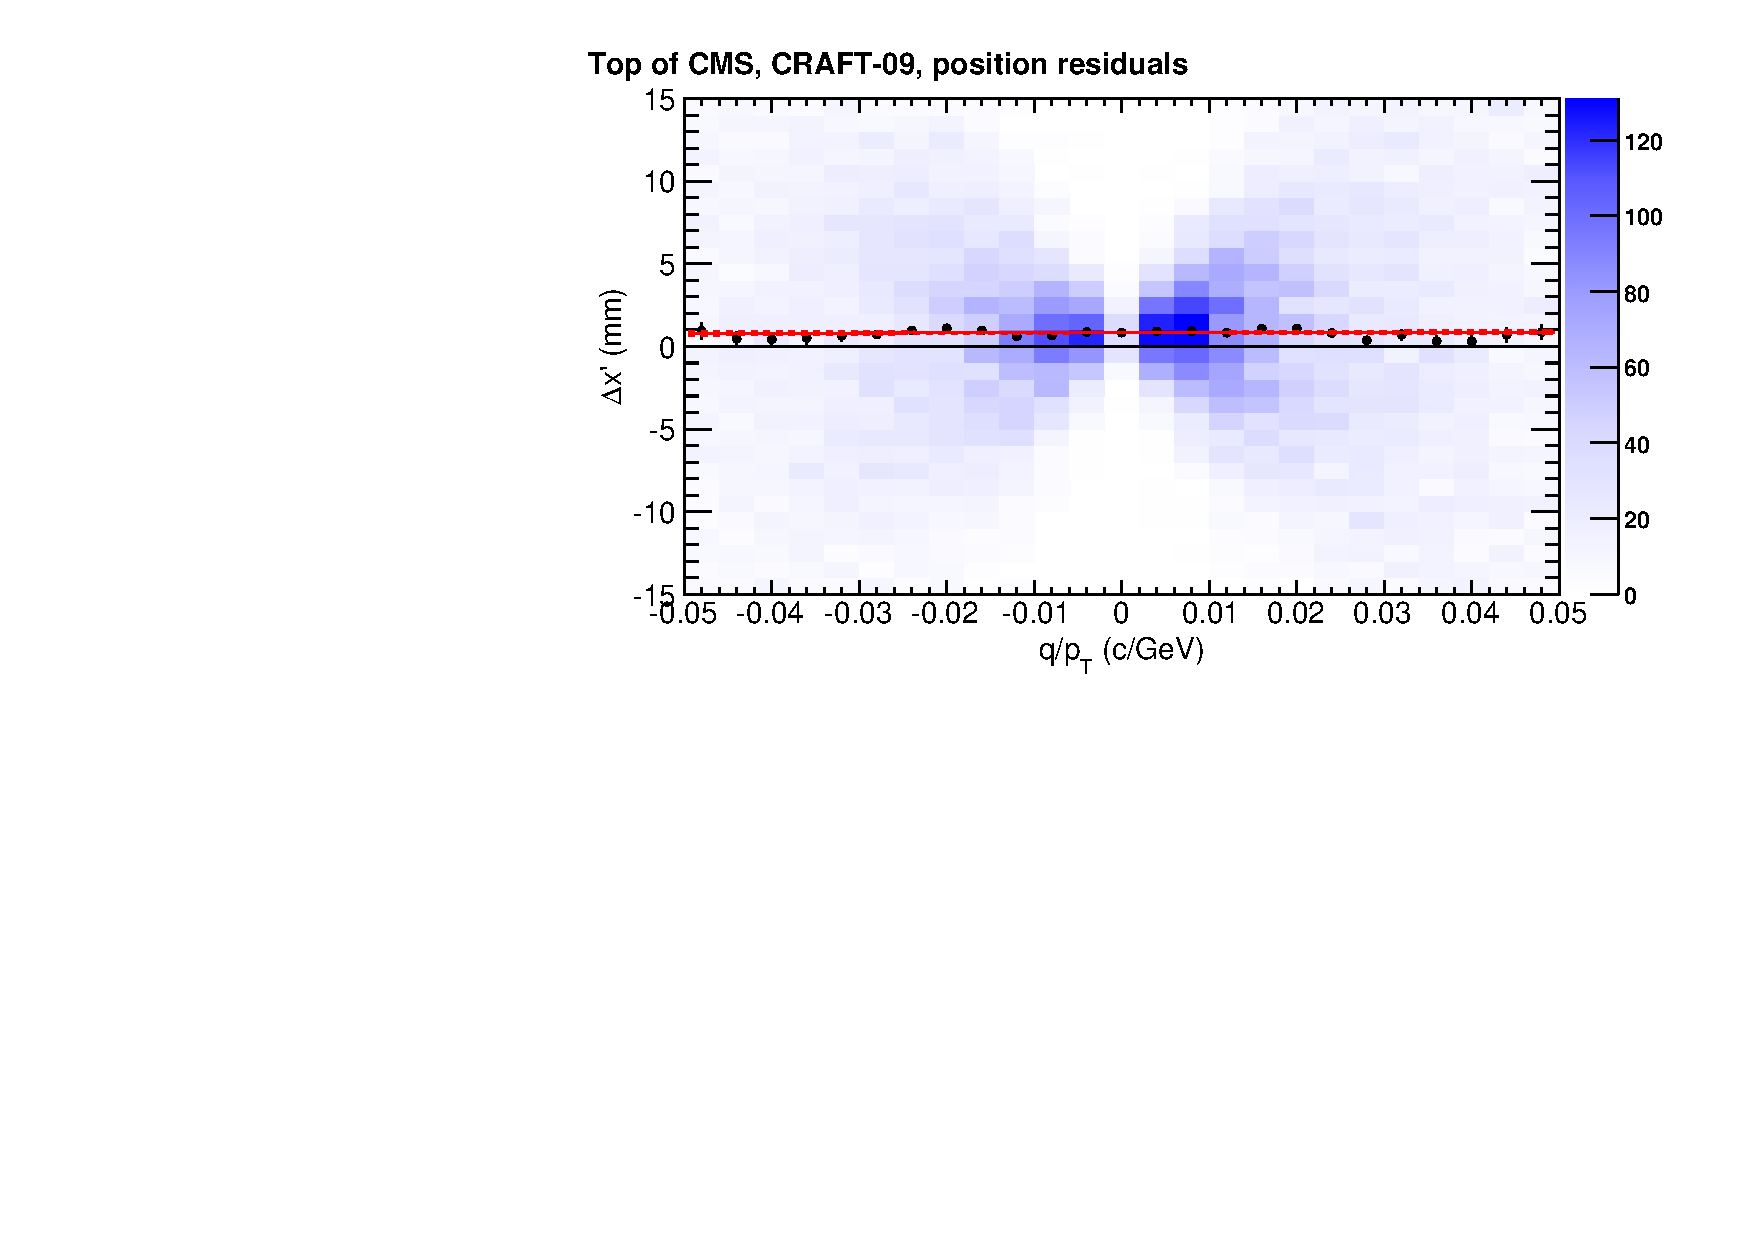
\includegraphics[width=\linewidth]{bfield_x_craft09_top.pdf} & 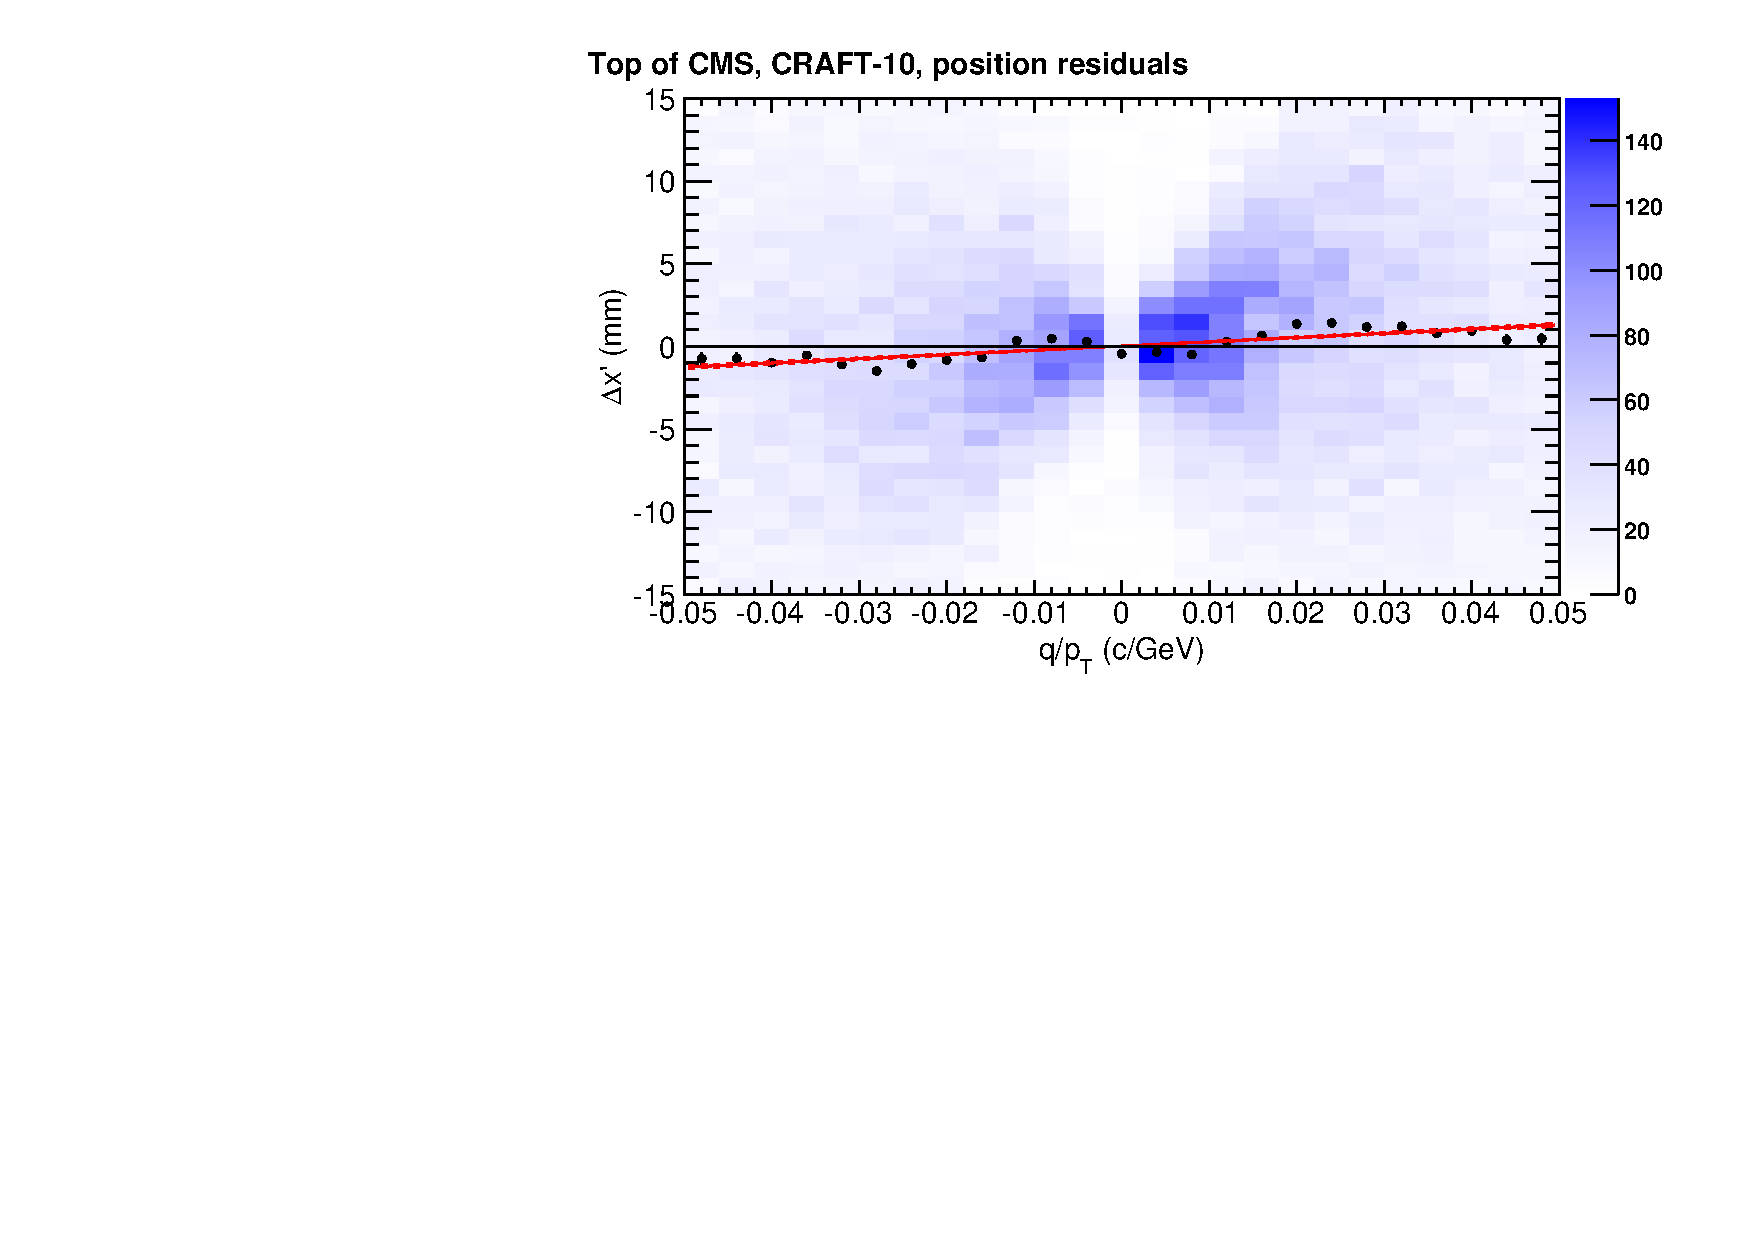
\includegraphics[width=\linewidth]{bfield_x_craft10_top.pdf} \\
\small \mbox{Top: $0.07 \pm 0.23$~cm$\cdot$GeV/$c$\hspace{-1 cm}} & \small \hfill \mbox{$2.57 \pm 0.18$~cm$\cdot$GeV/$c$} \\
& \\
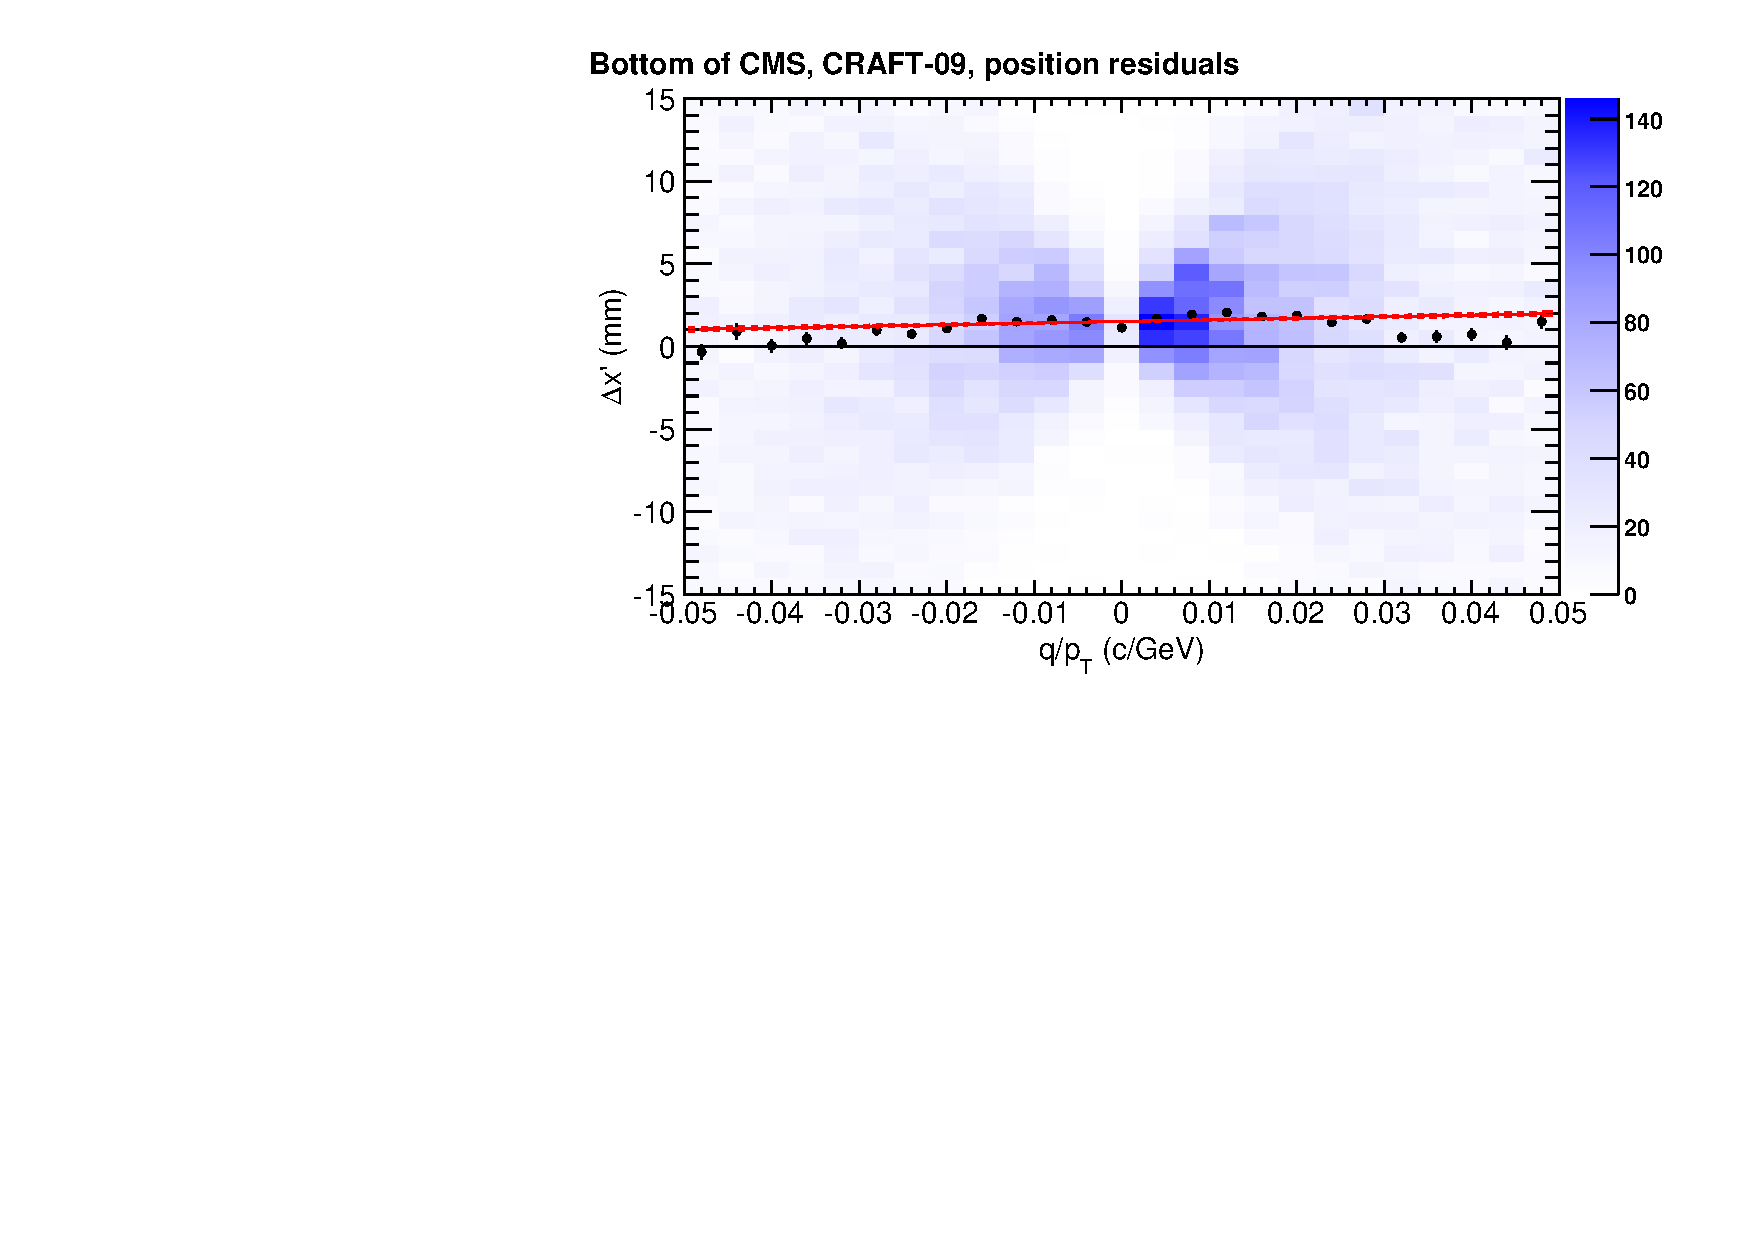
\includegraphics[width=\linewidth]{bfield_x_craft09_bottom.pdf} & 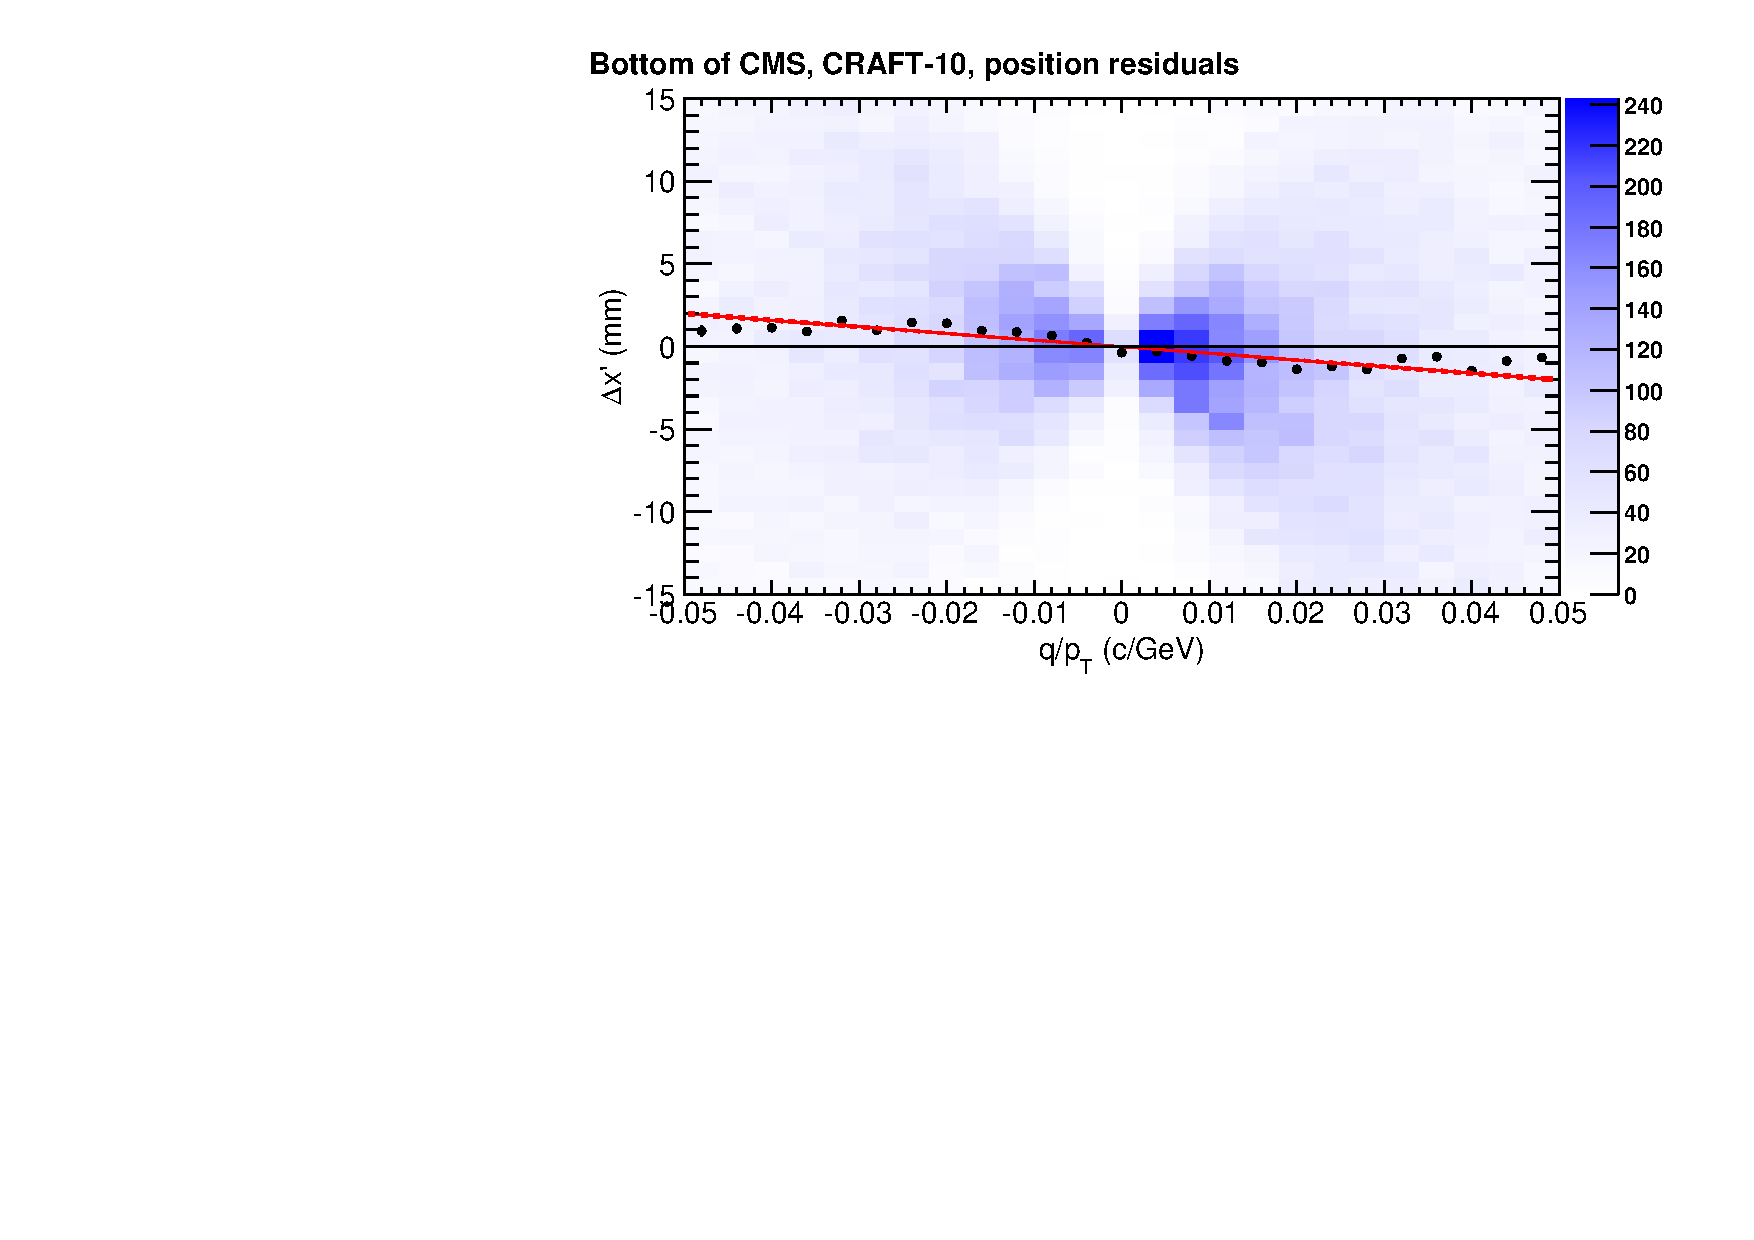
\includegraphics[width=\linewidth]{bfield_x_craft10_bottom.pdf} \\
\small \mbox{Bottom: $0.97 \pm 0.22$~cm$\cdot$GeV/$c$\hspace{-1 cm}} & \small \hfill \mbox{$-4.02 \pm 0.16$~cm$\cdot$GeV/$c$} \\
\end{tabular}
\end{frame}

\begin{frame}
\frametitle{\large Angle resids: \textcolor{black}{$\displaystyle \frac{\Delta dx'/dz}{q/p_T} = \int \frac{\Delta B_z(\ell)}{\mbox{330~cm}} d\ell$}}

\begin{tabular}{p{0.45\linewidth} p{0.45\linewidth}}
\begin{center} \large \textcolor{darkblue}{CRAFT-09} \end{center} & \begin{center} \large \textcolor{darkblue}{CRAFT-10} \end{center} \\
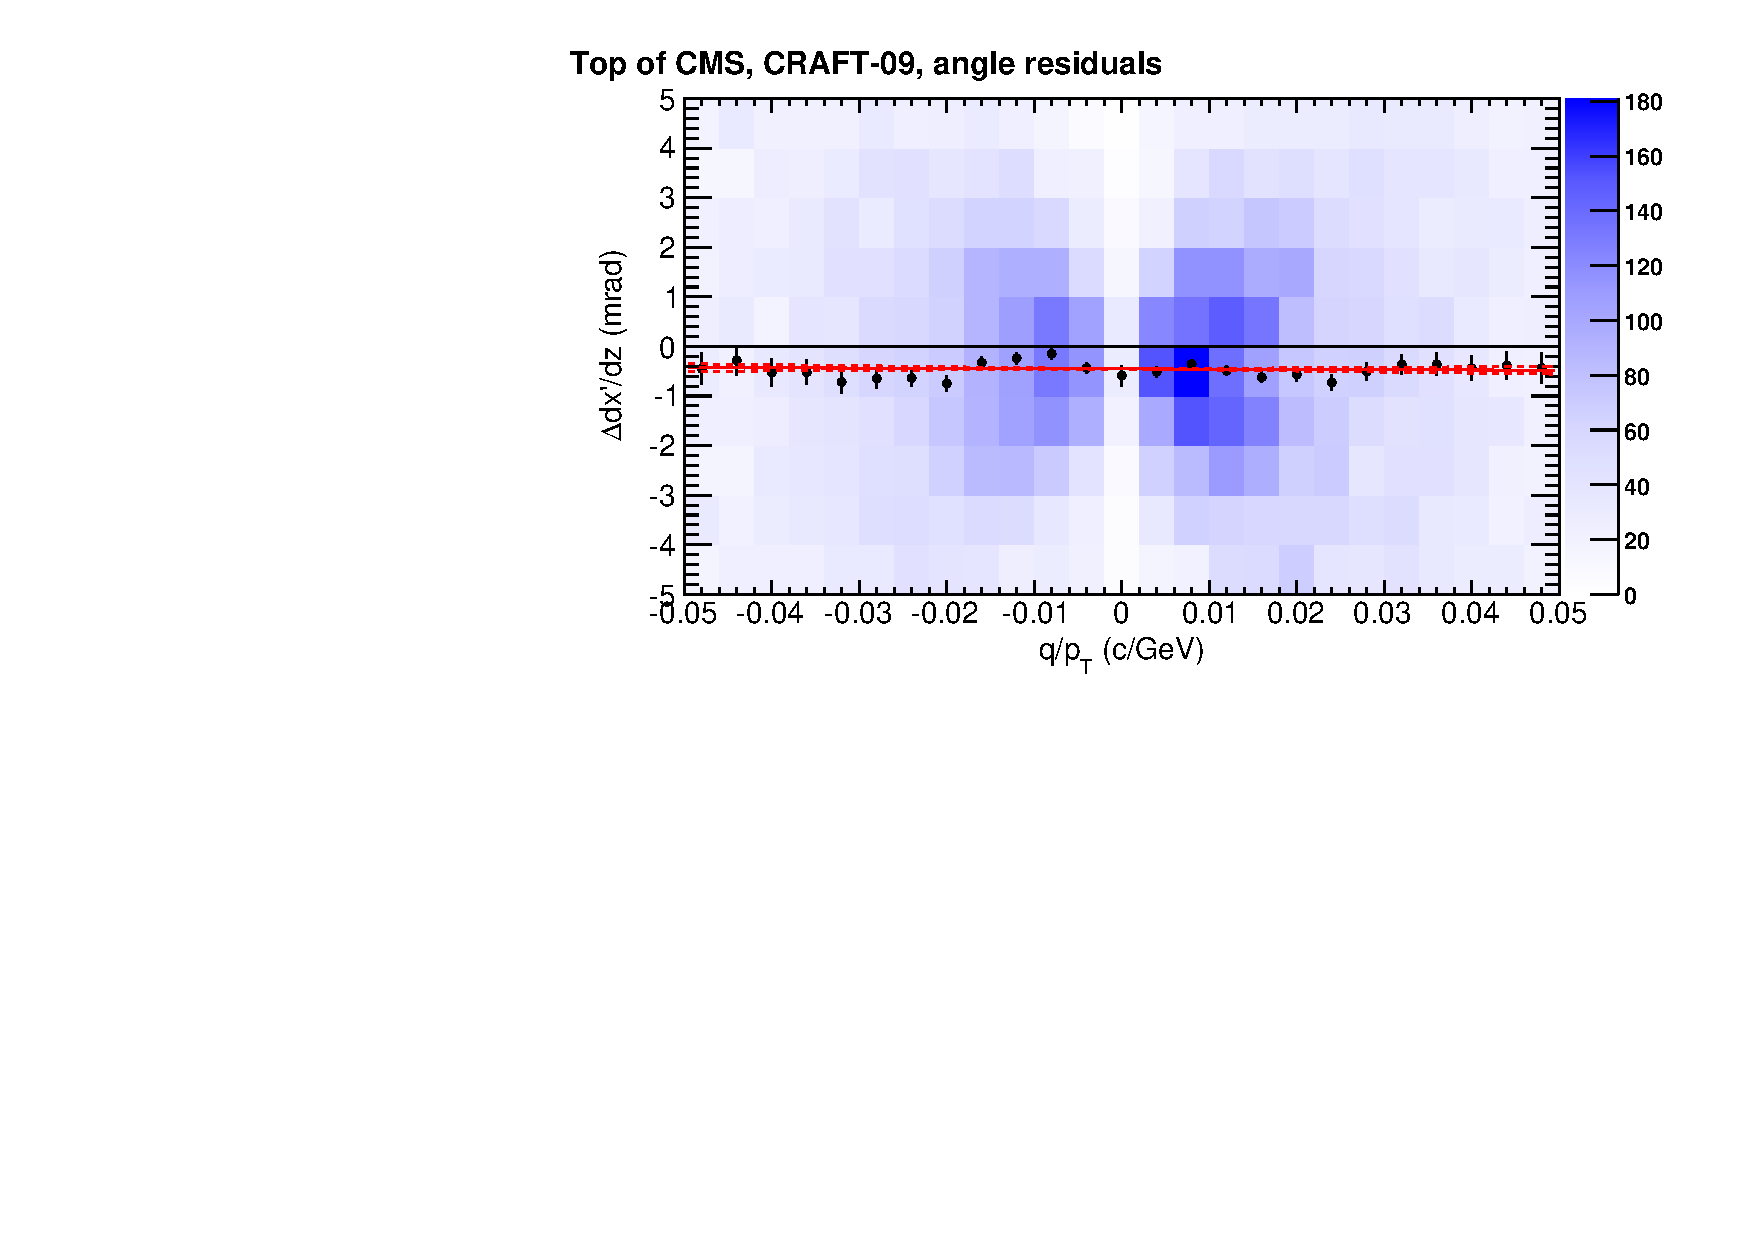
\includegraphics[width=\linewidth]{bfield_dxdz_craft09_top.pdf} & 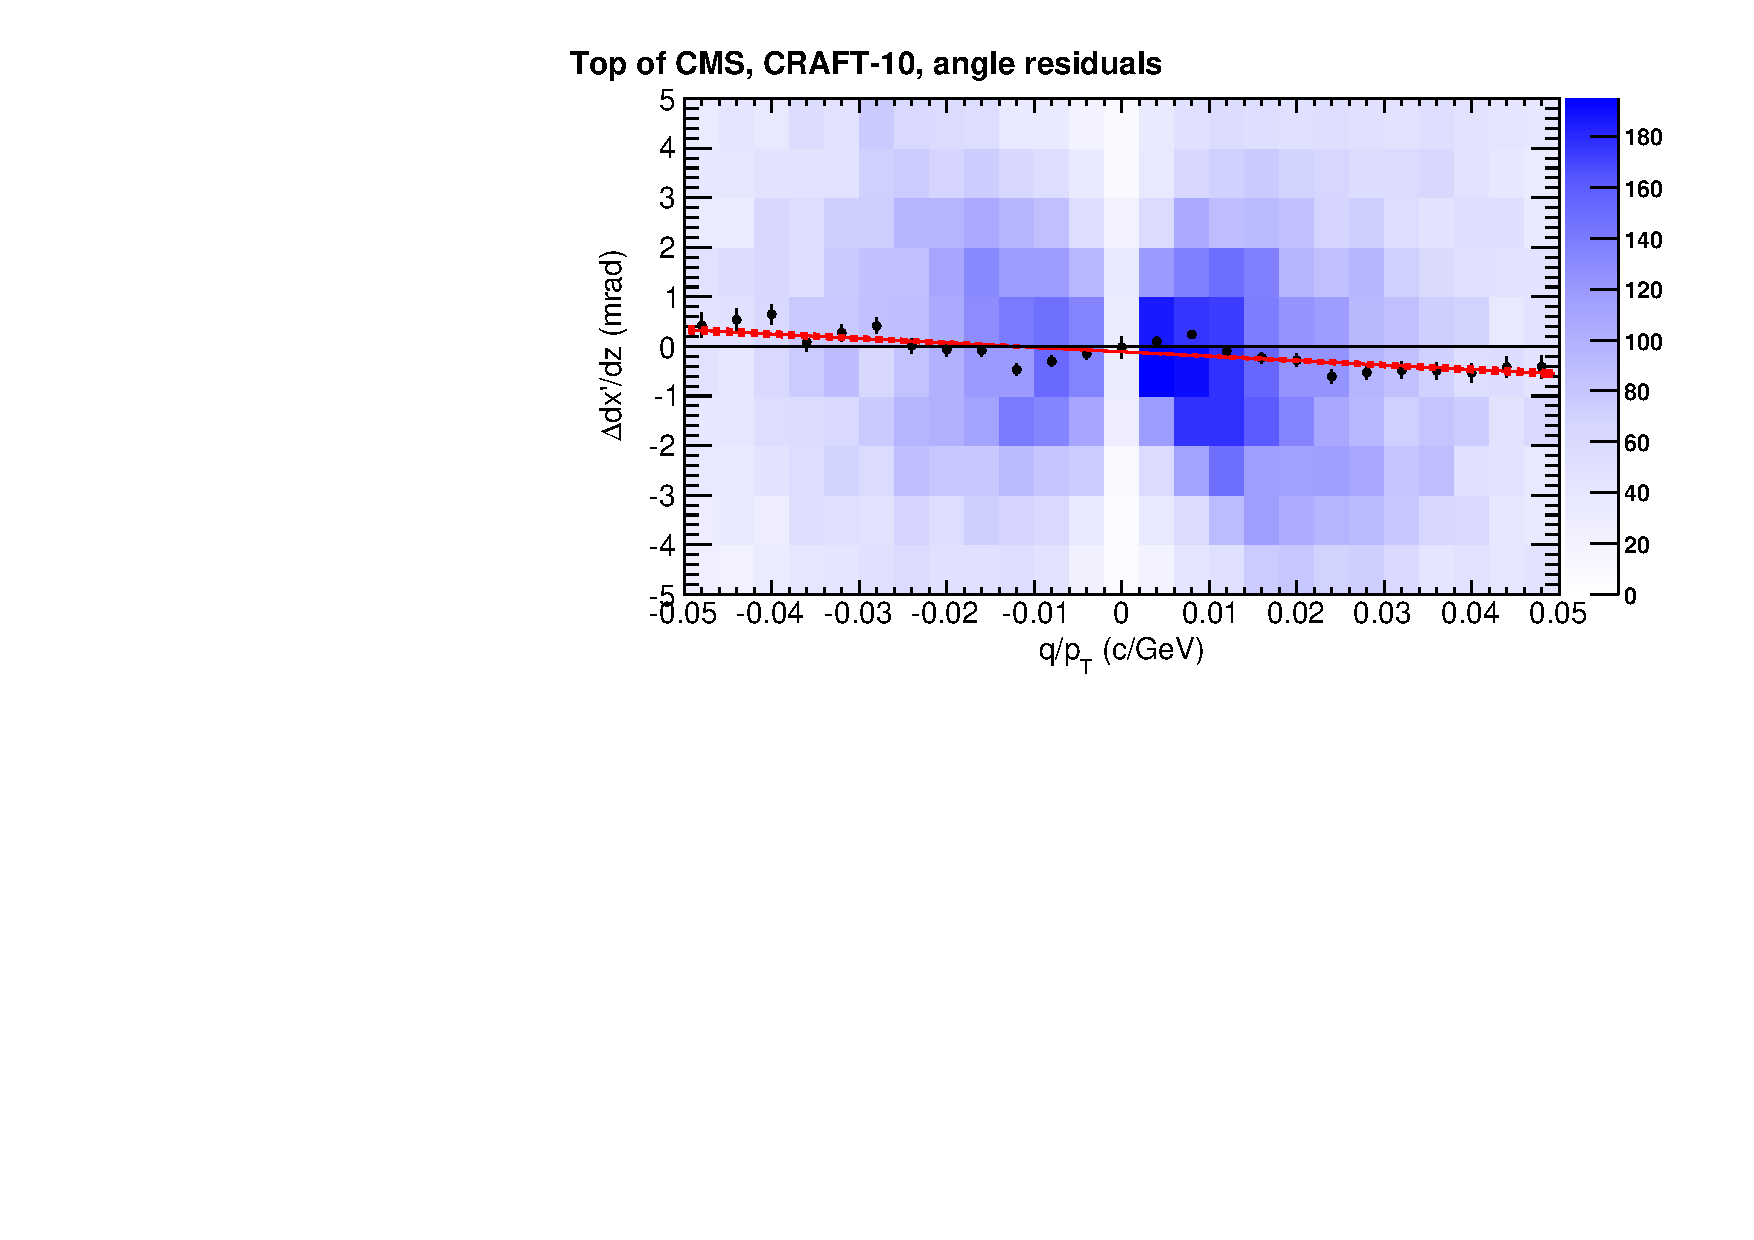
\includegraphics[width=\linewidth]{bfield_dxdz_craft10_top.pdf} \\
\small \mbox{Top: $-0.0005 \pm 0.0015$~rad$\cdot$GeV/$c$\hspace{-1 cm}} & \small \hfill \mbox{$-0.0089 \pm 0.0013$~rad$\cdot$GeV/$c$} \\
& \\
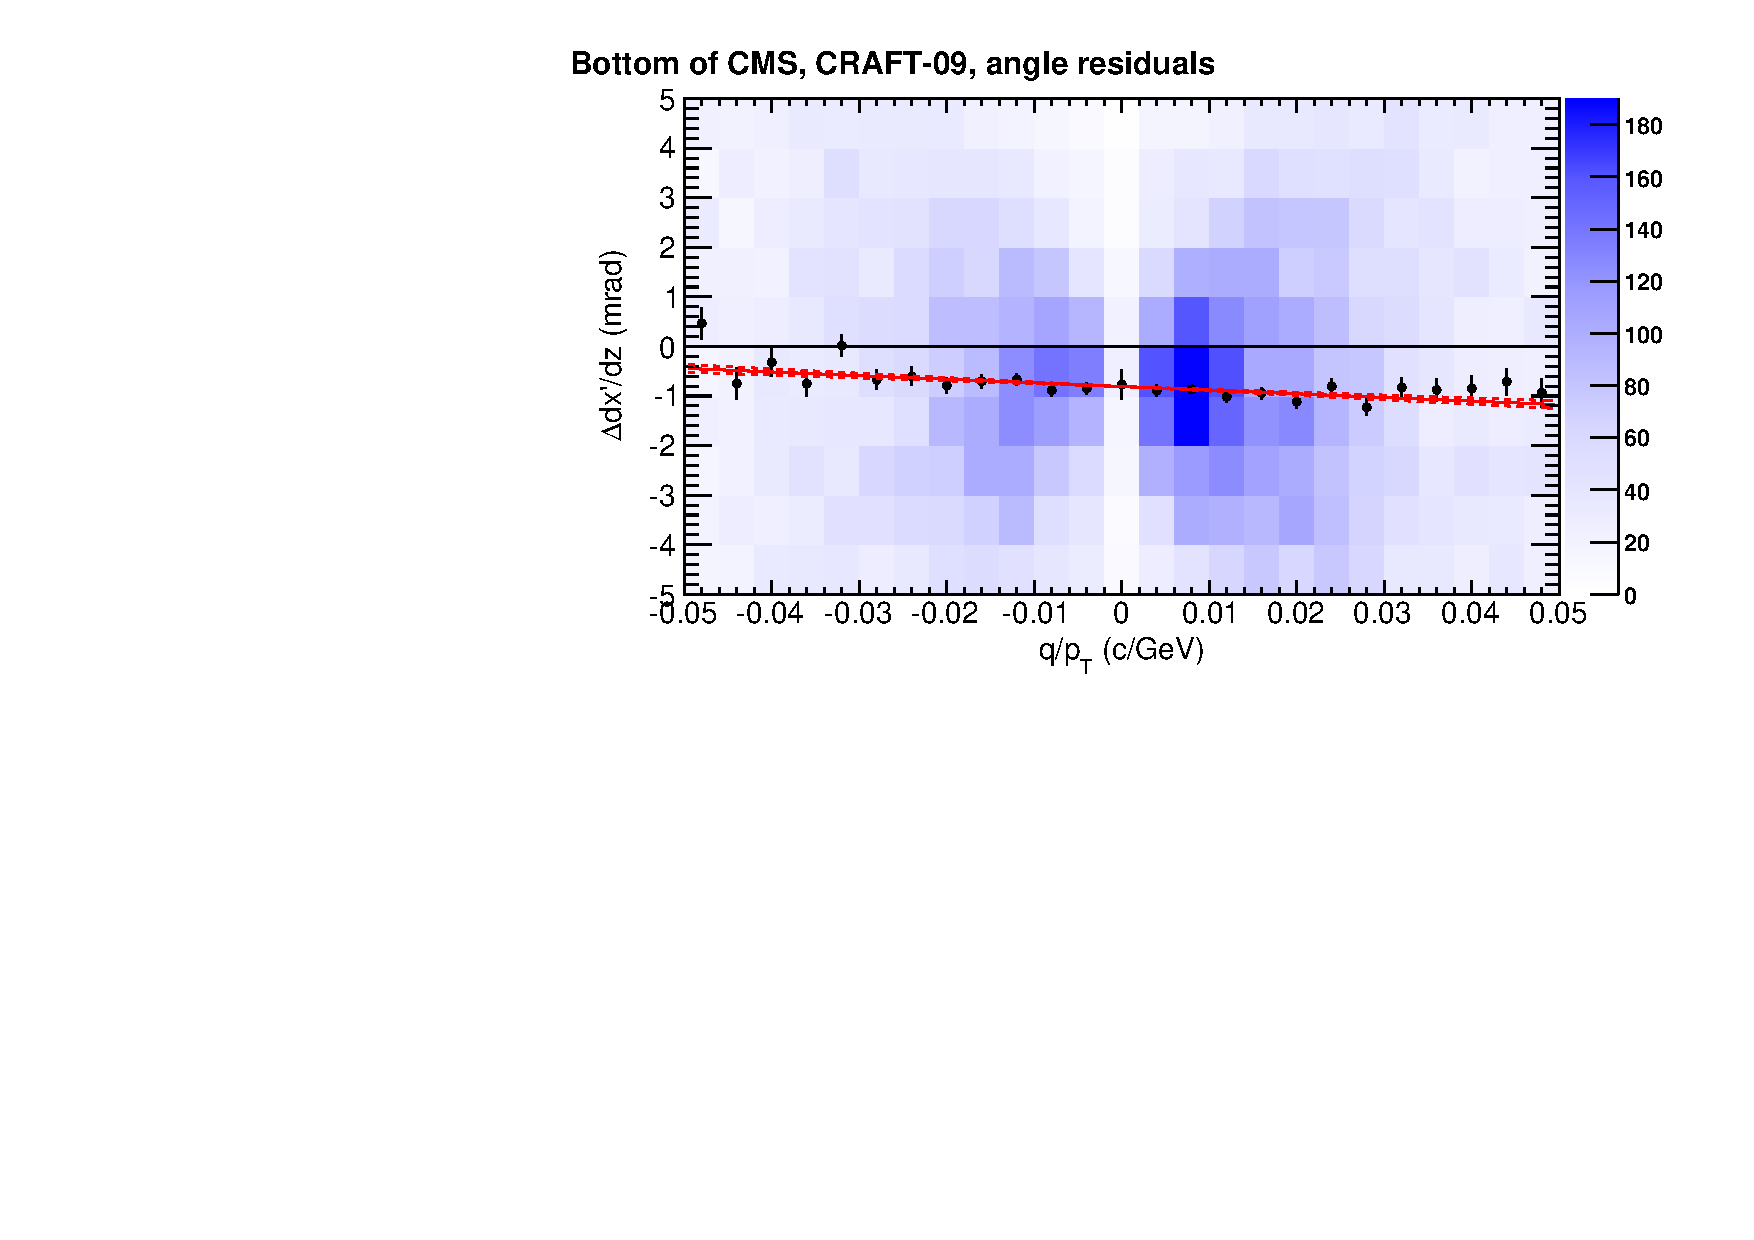
\includegraphics[width=\linewidth]{bfield_dxdz_craft09_bottom.pdf} & 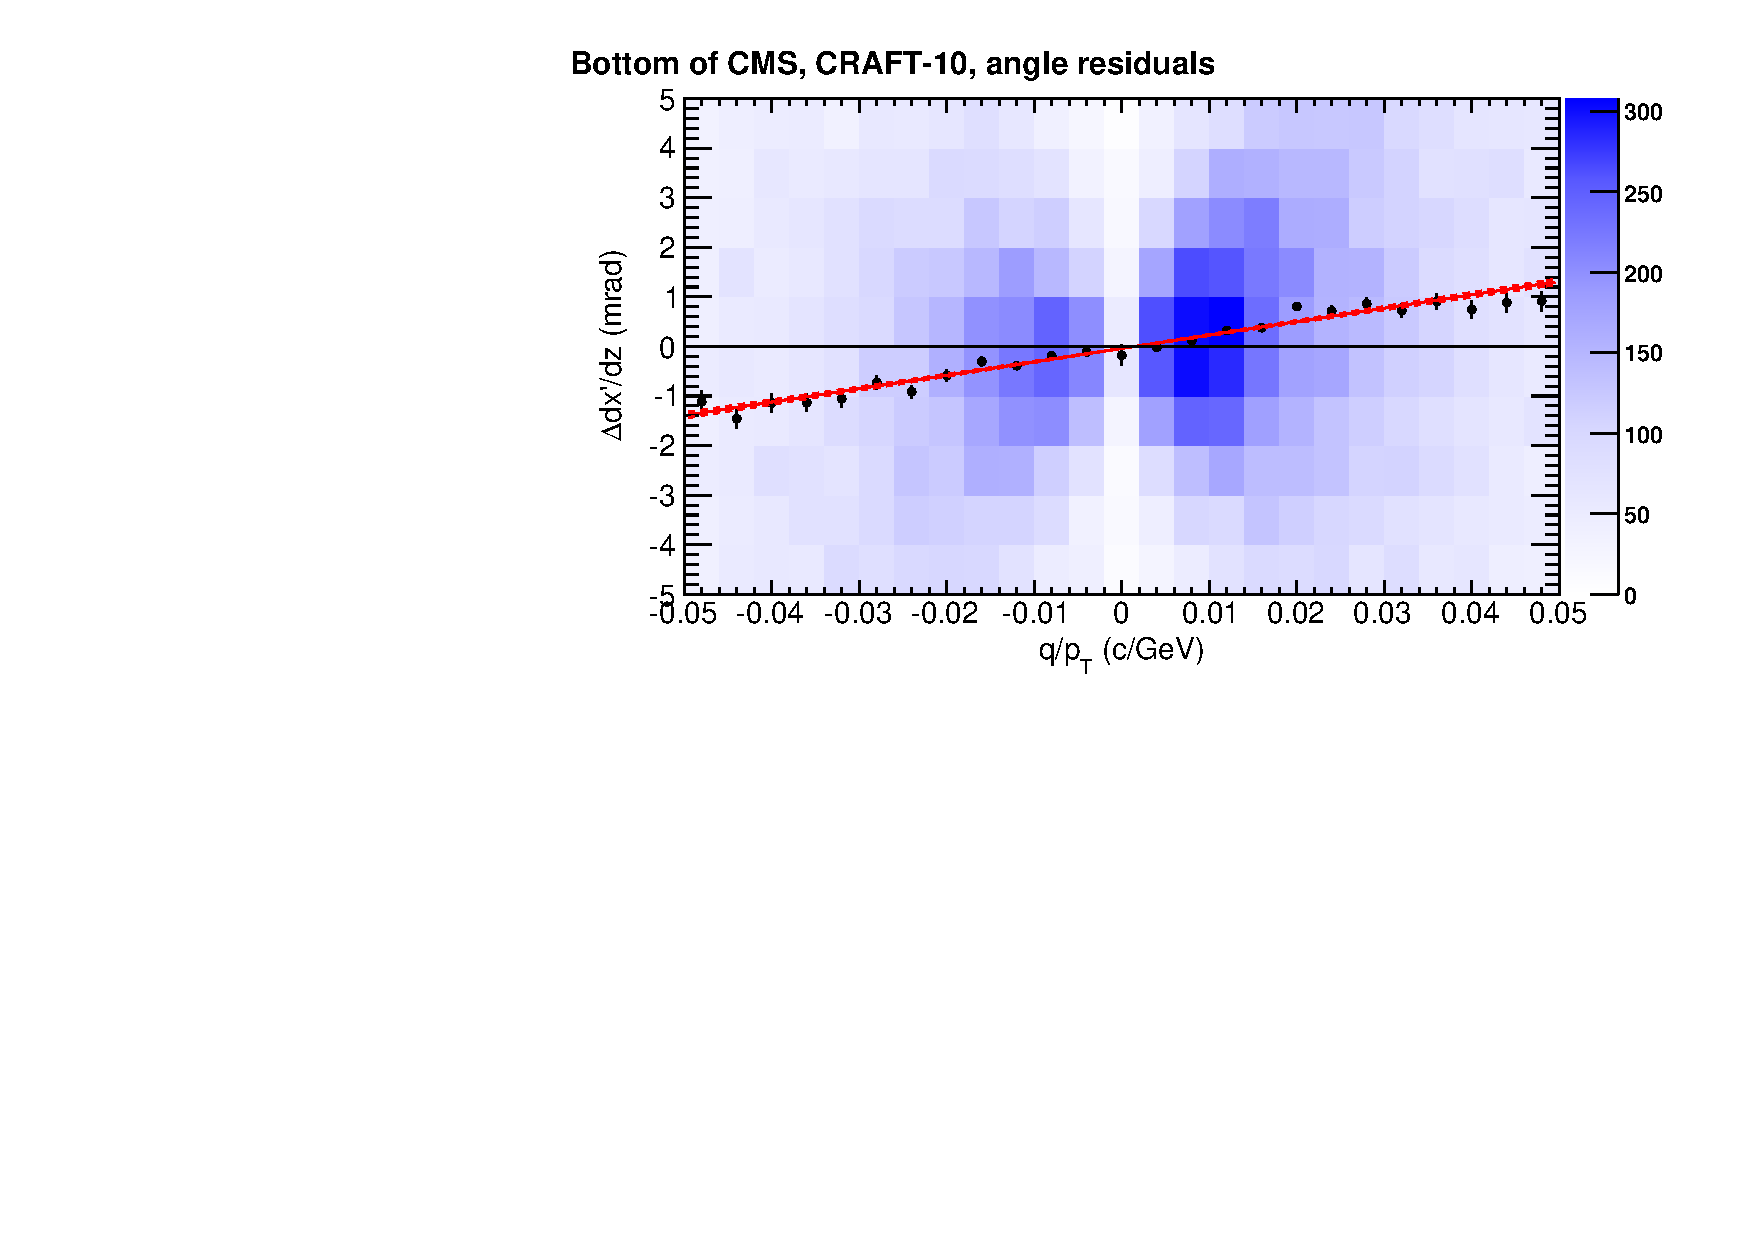
\includegraphics[width=\linewidth]{bfield_dxdz_craft10_bottom.pdf} \\
\small \mbox{Bottom: $-0.0073 \pm 0.0015$~rad$\cdot$GeV/$c$\hspace{-1 cm}} & \small \hfill \mbox{$0.0271 \pm 0.0011$~rad$\cdot$GeV/$c$} \\
\end{tabular}
\end{frame}

\begin{frame}
\frametitle{Individual chambers (angle resids)}

\begin{itemize}
\item If each chamber is fitted individually, the top slopes (1--6) are
  self-consistent and the bottom slopes (7--12) are self-consistent
\end{itemize}

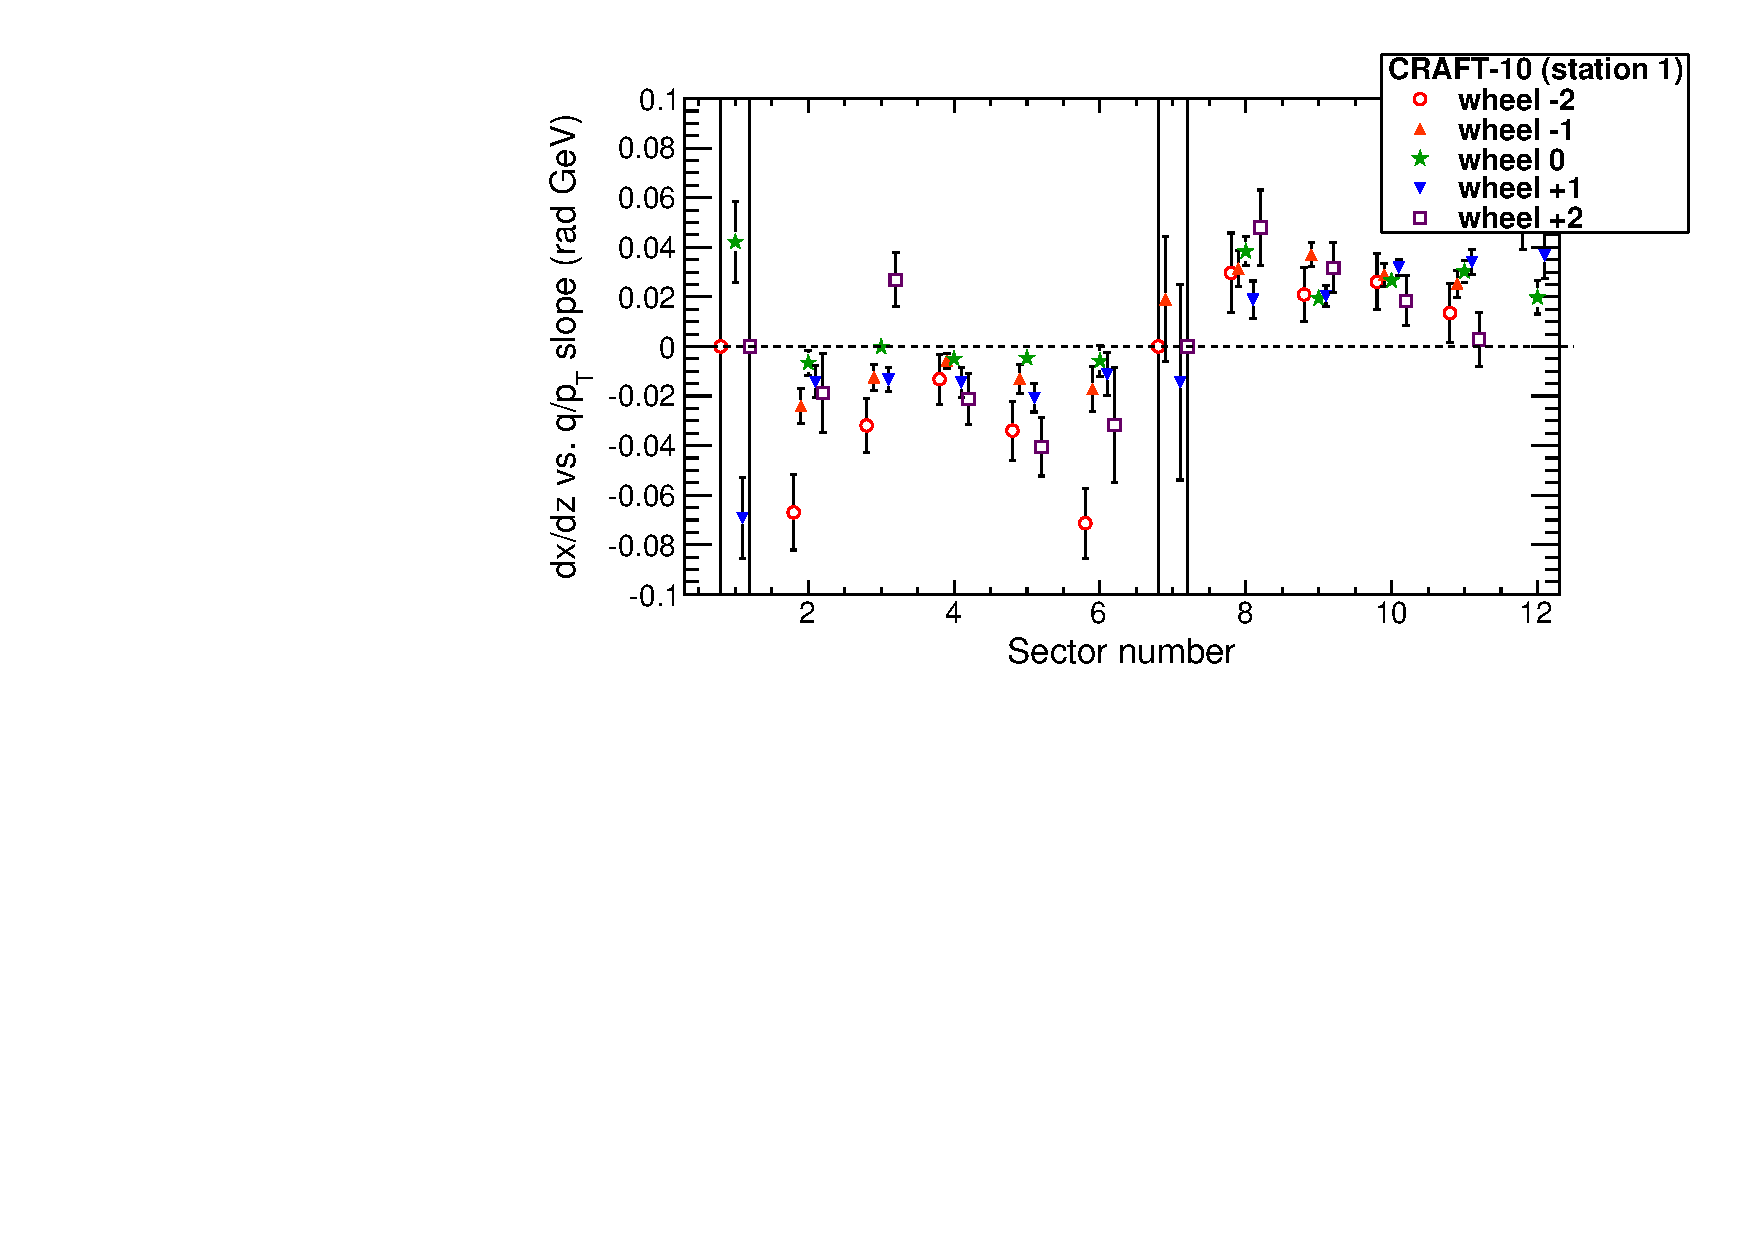
\includegraphics[width=0.8\linewidth]{bfield_dxdz_craft10_slopes_nosignswitch.pdf}

\begin{itemize}
\item Assuming $\displaystyle \int \Delta B_z(\ell) d\ell = \Delta B_z \times \mbox{210~cm}$,
\begin{itemize}
\item $| \Delta B_z| = 0.014$~T on top \hfill 0.3\% of 3.8~T
\item $| \Delta B_z| = 0.043$~T on bottom (same sign) \hfill 1.1\% of 3.8~T
\end{itemize}
\end{itemize}
\end{frame}

\begin{frame}
\frametitle{Station-to-station differences}

\begin{columns}
\column{0.5\linewidth}
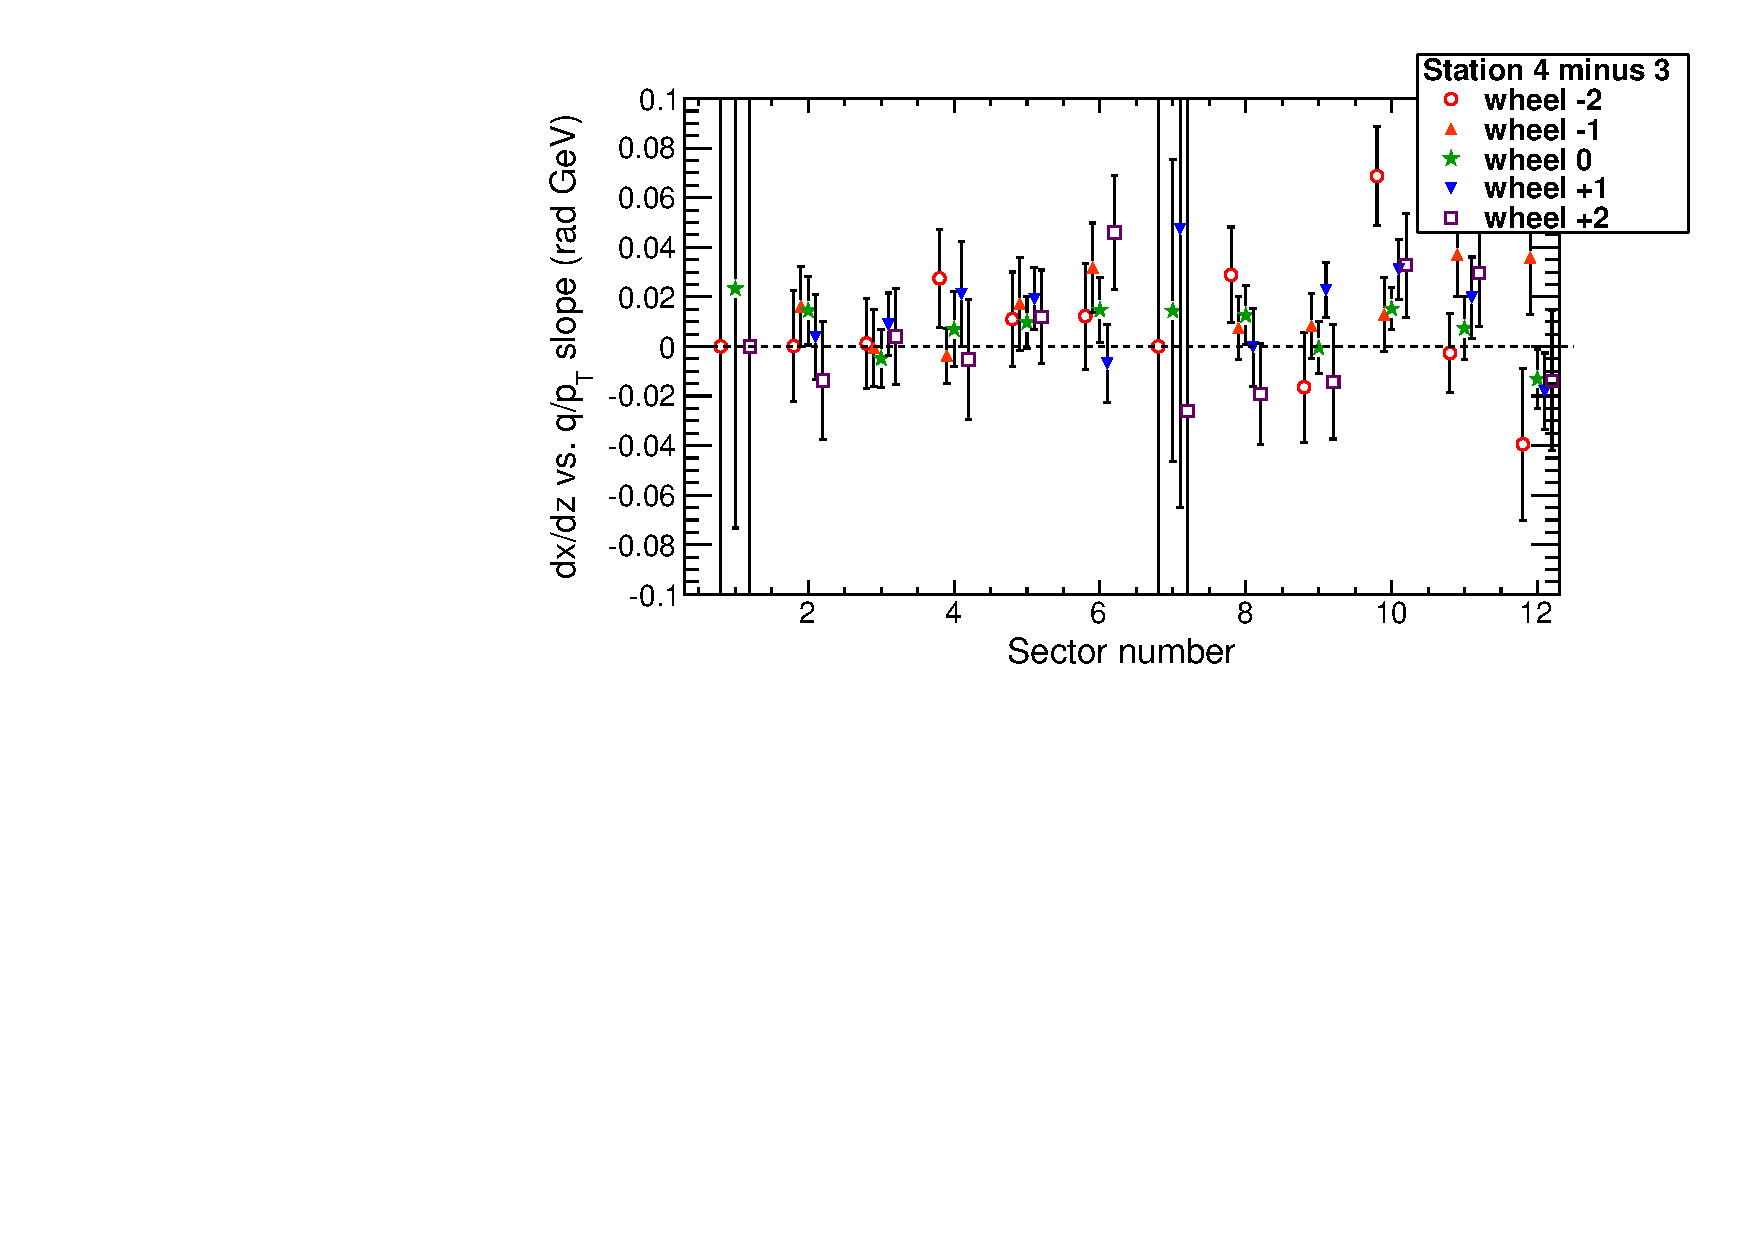
\includegraphics[width=\linewidth]{bfield_dxdz_slopes_nosignswitch_34.pdf}

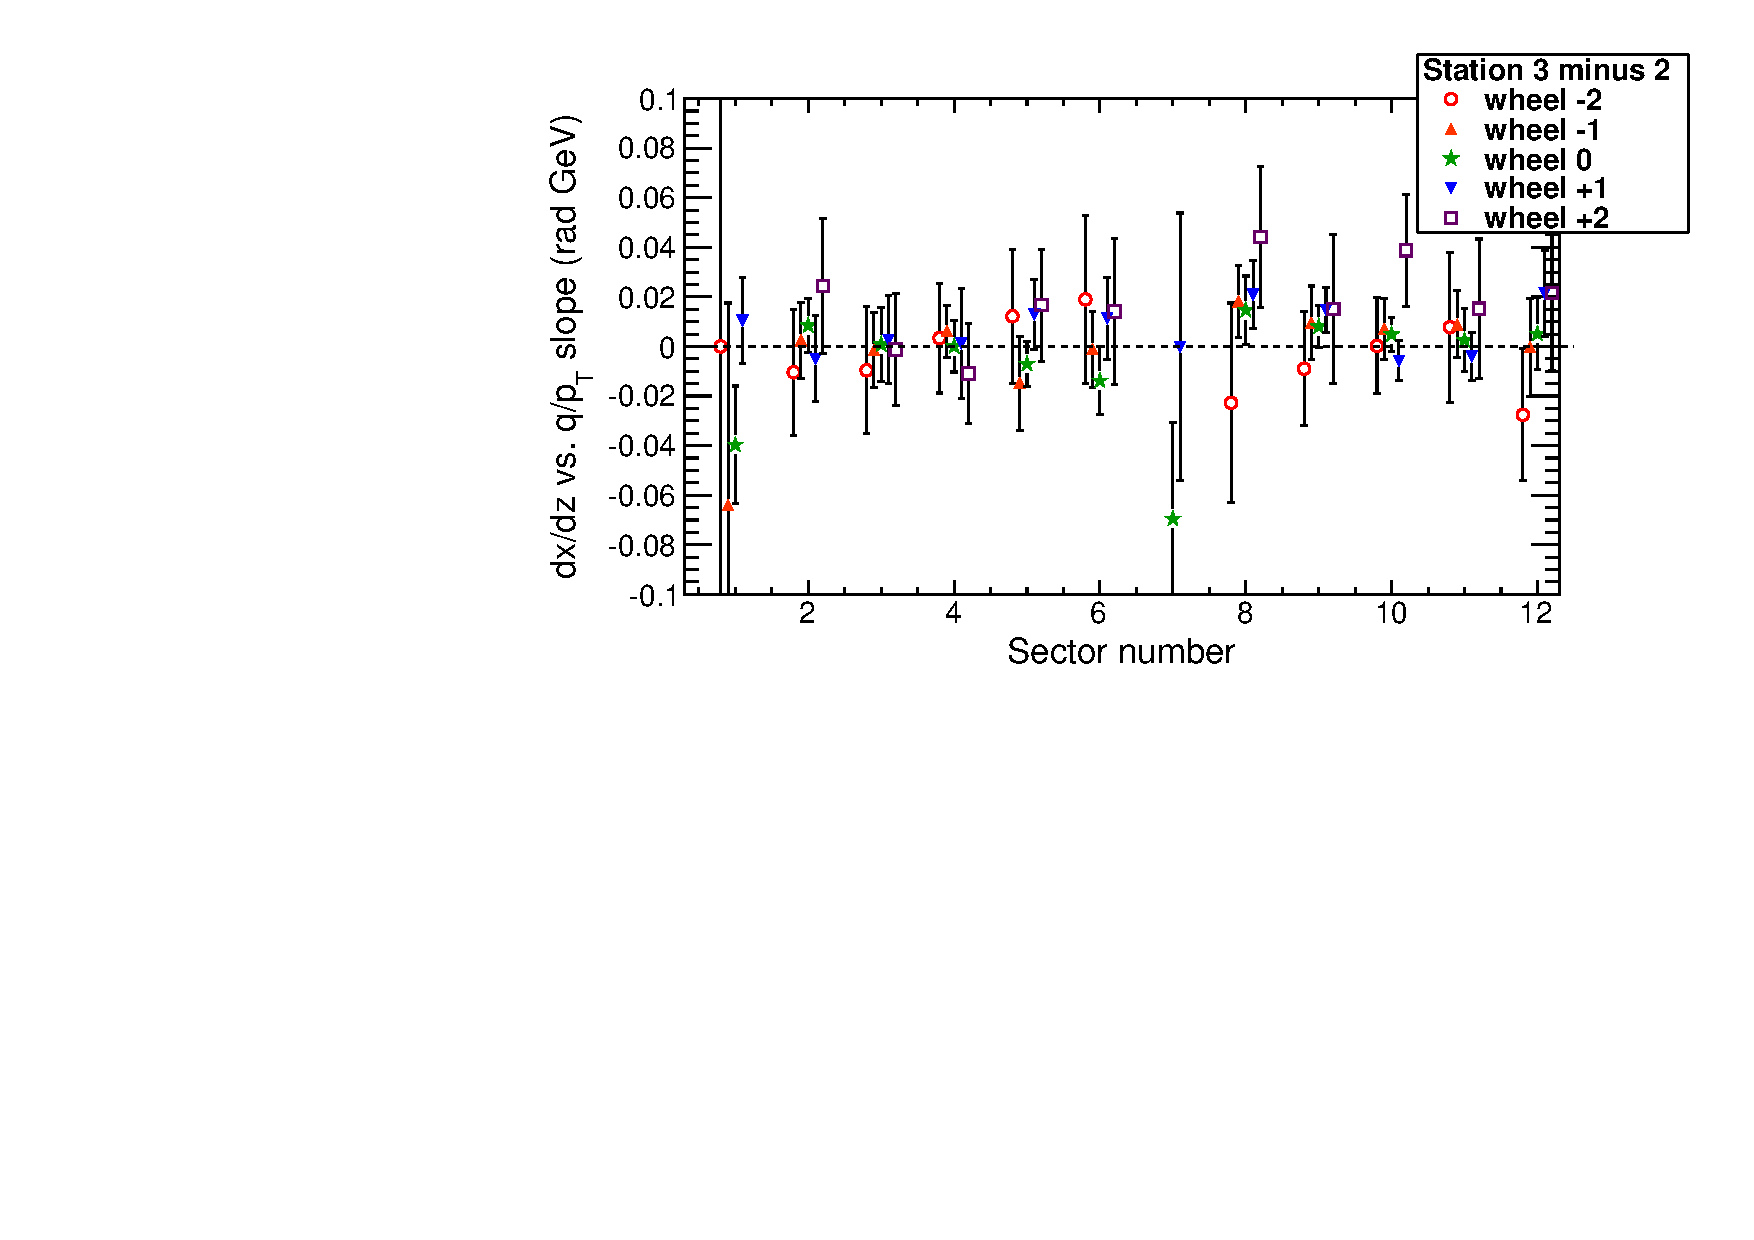
\includegraphics[width=\linewidth]{bfield_dxdz_slopes_nosignswitch_23.pdf}

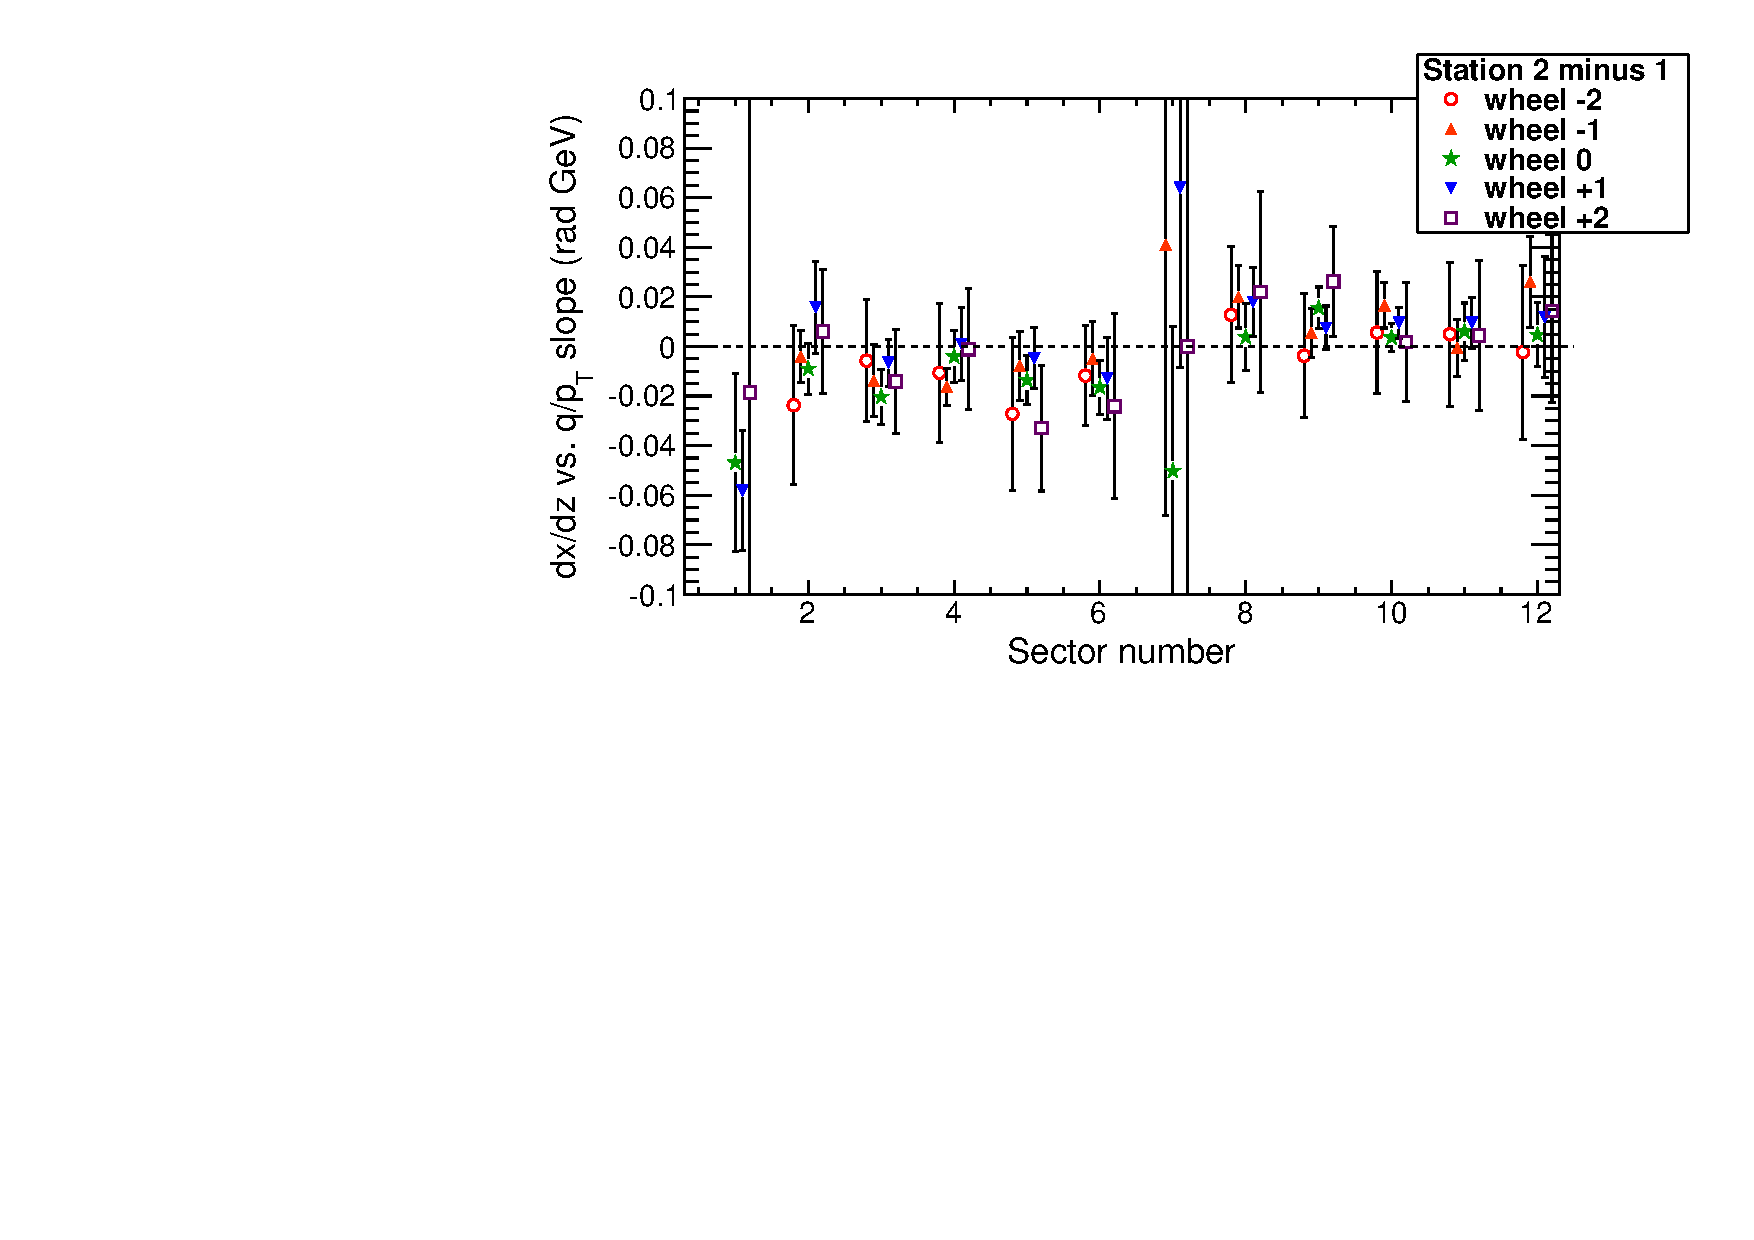
\includegraphics[width=\linewidth]{bfield_dxdz_slopes_nosignswitch_12.pdf}

\column{0.5\linewidth}
\begin{itemize}
\item For each track, subtract $\Delta \frac{dx'}{dz}$ in station $N$ from $\Delta \frac{dx'}{dz}$ in station $N+1$

\item Quantifies magnetic field error {\it between} stations

\item Only MB1 $\to$ MB2 is non-zero \\ ($\sim 0.01$ rad$\cdot$GeV/$c$)

\item Assuming $\displaystyle \int \Delta B_{z, 1\to 2}(\ell) d\ell = \Delta B_{z, 1\to 2} \times \mbox{20~cm}$
\begin{itemize}
\item $| \Delta B_{z, 1\to 2}| \sim 0.16$~T
\end{itemize}
\end{itemize}
\end{columns}
\end{frame}

%% \section*{First section}
%% \begin{frame}
%% \begin{center}
%% \Huge \textcolor{blue}{First section}
%% \end{center}
%% \end{frame}

\begin{frame}
\frametitle{Conclusions}

\begin{itemize}
\item RPC hits were included in alignment track refits by mistake, biasing the residuals
\begin{itemize}
\item removing these hits eliminates nearly all unexplained features
\item one correction resolves many mysteries, some of them years old
\end{itemize}
\item Effect on muon chamber alignment is $\mathcal{O}(\mbox{1--2 mm})$ with a systematic trend (rotation around beamline)
\item Muon residuals do not constrain tracker weak modes
\item We confirm the momentum scale bias seen by Pablo in CRAFT-10
\begin{itemize}\setlength{\itemsep}{0.1 cm}
\item {\it not} observed in CRAFT-09
\item interpreted as a $\vec{B}$-field error, it would have to be something that {\it changed} recently
\item $\sim$0.5\% offset in $Z$ mass for barrel standAloneMuons only ($\sim$0.1\% offset in barrel standAlone $J/\psi$)
\end{itemize}
\item Tangential observation: RPC hits cause a linear trend in
  $\Delta x$ vs.\ $x$, which could imply that the size of RPC chambers
  is incorrectly modeled by about 5~mm (instead of DTs, as we originally thought)
\end{itemize}

\label{numpages}
\end{frame}

\end{document}
